% Chapter 2, version 1 (02V1.tex): 21 September 2026.
% Supersedes the supplied 02V0(1).tex. Existing active section labels retained once.
% Required packages: amsmath, graphicx, booktabs, array, tabularx, natbib.
% Figure: Images/CH02_MassRank_V1.pdf (supplied with this revision).
% References: merge Chapter_02_References_V1.bib by citation key; do not duplicate keys.
% Calibration thresholds and incomplete experiments are not presented as completed.

\chapter{Literature Review}
\label{ch:litreview}

% \section{Introduction}
% \label{sec:lr-intro}

% A forgery detector neural network pipeline can make the correct decision between bona-fide and forged identification document(ID) while giving a poor indication on the spatial map, as to where the alteration lies. This chapter reviews the literature needed to investigate whether an adversary can create that failure from an initially useful spatial map. This included research into identity-document datasets, spatial map generation techniques including post-hoc attribution and native localisation, and attacks on spatial outputs. It then explains the choice of relevance mass and rank accuracy, and how these established metrics and measures support this study's DC--DCEC--DCEW framework.

% The review connects findings to the research choices they support. Dataset and pipeline selection inform the clean baselines in O1; limitations of spatial measures inform the audit and calibration in O2; adversarial studies inform O3 and O4. Its scope is a focused critical review of these connected areas. The research gap concerns a particular conditional failure, rather than a claim that spatial maps have not previously been attacked.

\section{Introduction} \label{sec:lr-intro} A forgery detector neural network pipeline can make the correct decision between bona-fide and forged identity document (ID) while giving a poor indication on the spatial map, as to where the alteration lies. This distinction is particularly important because IDs have many semantically distinct regions such as portraits, biographical text and document identifiers, coexisting with graphical and security features that are issuing authority specific. ID forgery may affect anything from a small part of a textual field to an entire portrait. 

Before considering attacks on spatial evidence, it is therefore necessary to establish the characteristics of ID forgery as a forensic problem. This chapter reviews the literature needed to investigate whether an adversary can degrade an initially useful spatial map while preserving the detector's forgery decision. It considers the domain-specific characteristics of manipulated IDs and the datasets available for studying them. 

It then reviews two routes to spatial evidence followed by methods for evaluating spatial agreement and adversarial work targeting spatial outputs. These strands motivate the use of relevance mass and relevance rank accuracy and support this study's DC--DCEC--DCEW framework. 

The review connects findings to the research choices they support. 
\begin{enumerate}[itemsep=1pt]
    \item Dataset and pipeline selection inform the clean baselines in O1
    \item Limitations of spatial measures inform the audit and calibration in O2
    \item Adversarial studies inform O3 and O4.
\end{enumerate}

Its scope is therefore a focused critical review of the literature needed to examine whether spatial evidence that is acceptable on a correctly detected forged ID can be degraded without changing the forgery decision. The research gap is this domain-specific conditional failure evaluation rather than a claim that spatial maps have not previously been attacked.

% \section{Manipulated identity document as a forensic problem}
% \label{sec:lr-context}

% In remote verification, software often examines a photograph of a document. A digitally replaced portrait or an edited date of birth can therefore reach a detector without the attacker producing a convincing physical counterfeit. FantasyID models this digital-manipulation setting using face swapping and text inpainting \citep{korshunov2025fantasyid}. The later adversarial perturbation studied here is a separate change to that already manipulated image.

% Hence in the remote verification, two naturally arising questions are:
% \begin{enumerate}
%     \item Whether the document is forged
%     \item Whether detectors pipeline's spatial output directs attention towards the alteration.
% \end{enumerate}

% Neither answer establishes how a person using remote verification pipeline in banking or law enforcement agencies will use the map. NIST's Explainable AI principles distinguishes an explanation that is user-centric and understandable from an explanation that embeds model fidelity and accurately reflects the system's process \citep{phillips2021four}. This distinction motivates careful evaluation, but annotation agreement alone cannot demonstrate explanation faithfulness or improved human in the loop's decisions. The present study evaluates spatial agreement. It does not test a banking verification service or its reviewers.

%--------------------------------------------------------------------------------------------------
\section{Identity-document forgery as a domain-specific forensic problem} \label{sec:lr-context} 

International specifications for machine-readable travel documents define standards for physical dimensions, visual data layouts, and machine-readable zones to ensure global interoperability. The framework also addresses guidelines for protecting biographical data against alteration and establishes electronic chip and cryptographic standards \citep{icao9303}. For certification of remote verification software, FIDO's standardised test criteria include features such as holograms, guilloché patterns, microprinting, ghost images, specialised fonts, and interactions between the primary portrait and the document background \citep{fido2026docauth}. 

Consequently, IDs are a structured security artefact but not all of the physical security properties are observable from a single digital photograph used in remote verification. Some features depend on illumination, viewing angle, wavelength or electronic access. Since remote verification commonly operates on captured or uploaded document images, it makes it possible for alterations to the visually observable identity fields to reach an automated detector without the attacker constructing a complete physical counterfeit. The forensic problem considered in this thesis is restricted to this digital-image setting. 

Within that setting, the spatial scale and semantic importance of a manipulation can vary substantially. Altering one or more characters in a date of birth, name or document number may modify only a very small image region while materially changing the represented identity. At the other extreme, a portrait may be partially modified or replaced entirely. The DeepID challenge identifies this combination of high-value targets including names, dates, identification numbers and facial portraits as a distinctive difficulty in ID manipulation detection, and treats document-level detection and pixel-level localisation as separate forensic tasks \citep{korshunov2025deepid}. FantasyID models the same digital-manipulation setting using face-swapping and text-inpainting attacks and provides annotations of the manipulated regions \citep{korshunov2025fantasyid}. 

These properties also affect the learning formulation. A generic whole-image representation need not explicitly encode that a small change inside a date field can have greater forensic significance than a visually larger change in an irrelevant background region. Recent field-localised work therefore argues for explicitly modelling semantically important regions such as portraits and textual fields rather than treating the entire document as homogeneous image content \citep{kumar2026flid}. 

By explicitly representing manipulation classes during training, supervised modelling enables the system to learn the domain structure directly from the available labels. This does not mean that unsupervised or self-supervised approaches are unsuitable for ID fraud. A purely closed-set supervised detector may fail to represent new document layouts, fabrication processes or previously unseen fraud strategies. Recent work on open-set ID-fraud discovery consequently combines document-specific representation learning with self-supervised and supervised objectives to identify anomalous and previously unseen fraud patterns \citep{li2026layoutaware}. Supervised detection and open-set anomaly discovery should therefore be viewed as complementary responses to different parts of the problem. 

The present study concerns known digital manipulation families for which labels and alteration regions are available, making supervised detection and explicit spatial evaluation appropriate to the research question. 

In remote verification pipelines, two naturally arising questions are: 
\begin{enumerate} [itemsep=1pt]
\item Does the pipeline correctly classify the document as forged? 
\item Does its spatial output direct evidence towards the known alteration? 
\end{enumerate} 

A correct answer to the first question does not imply a useful answer to the second. A detector may exploit document-wide acquisition or processing traces, or other predictive cues outside the altered field, and still produce the correct document-level decision. 

This separation between decision correctness and spatial agreement motivates the clean evidence conditions introduced later in this chapter. The adversarial perturbation studied in this thesis is a further, separate modification applied to an already forged image. Its purpose is not to create the underlying identity-document forgery, but to test whether initially acceptable spatial evidence can be degraded while the forgery decision is preserved.
%--------------------------------------------------------------------------------------------------
% \section{Datasets and the selection of FantasyID}
% \label{sec:lr-data}

% The dataset must provide complete document images and known manipulation regions. Capture conditions also matter because a forensic model may use processing traces that disappear in digitally rendered images. Table~\ref{tab:lr-datasets} compares the main alternatives against these requirements.

% \begin{table}[htbp]
% \centering
% \small
% \renewcommand{\arraystretch}{1.15}
% \caption{Dataset suitability for whole-document spatial evaluation. Limitations refer to the needs of this study.}
% \label{tab:lr-datasets}
% \begin{tabularx}{\textwidth}{@{}>{\raggedright\arraybackslash}p{0.23\textwidth}>{\raggedright\arraybackslash}X>{\raggedright\arraybackslash}X@{}}
% \toprule
% Dataset & Useful evidence & Main limitation here \\
% \midrule
% MIDV-2020 \citep{bulatov2022midv2020} & Mock documents across photographs, scans and videos. & Recognition benchmark without paired digital-forgery masks. \\
% SIDTD \citep{boned2024sidtd} & Extends mock documents with crop-and-replace and inpainting attacks. & Constructed templates and attack generation differ from the selected setting. \\
% IDNet \citep{guan2024idnet} & Large synthetic collection with varied document types and fraud patterns. & Digital renders do not reproduce the same physical capture history. \\
% FakeIDet2 / FakeIDet3-DB \citep{munozharo2026fakeidet2,munozharo2026fakeidet3} & Privacy-aware patches from real IDs; the newer release adds digital attacks. & Released patches do not preserve complete-document spatial context. \\
% FantasyID \citep{korshunov2025fantasyid} & Complete captured cards, face/text edits and region annotations. & Fictional layouts, approximate masks and repeated captures limit generalisation. \\
% \bottomrule
% \end{tabularx}
% \end{table}

% These alternatives address different problems. MIDV-2020 supports recognition under capture variation, while SIDTD adds forgery examples. IDNet prioritises scale through synthesis. FakeIDet2 brings real-document traces into a privacy-aware benchmark; FakeIDet3-DB extends this approach to classical and generative digital attacks. The large IDNet release and FakeIDet3-DB are described in preprints, so their reported capabilities warrant the same scrutiny as their useful data contributions.

% FantasyID offers the closest fit among these datasets: physical print-and-capture, complete images, portrait and text manipulations, and annotations. Its original study also reports substantial test errors at a validation-selected operating point, despite useful ranking performance \citep{korshunov2025fantasyid}. Thus, published detection performance does not establish that enough individual images have useful spatial evidence for an adversarial study. Clean eligibility must be measured directly.

% The DeepID challenge provides further identity-document evidence, including TruFor baselines and submissions evaluated on a private real-document set \citep{korshunov2025deepid}. That private evaluation cannot be reproduced from FantasyID alone. The challenge report also records a team's observation of different JPEG quality factors for bona-fide and manipulated images. This motivates a compression audit, rather than assuming that a correct decision necessarily reflects the edited field. Shortcut learning offers the broader explanation: models can exploit predictive features that fail outside the training setting \citep{geirhos2020shortcut}.

% Three limitations remain after dataset selection. Rectangular annotations approximate the altered regions; capture variants of one card are dependent observations; and fictional documents cannot establish performance across real issuing authorities. These motivate mask-sensitivity checks, grouping by document stem and restricted claims. Chapter~3 defines these controls; Appendix~A records metric-related risks and the model-specific registers retain preprocessing decisions.

%--------------------------------------------------------------------------------------------------

\section{Datasets, assurance criteria and the selection of FantasyID}
\label{sec:lr-data}

Dataset selection is a trade-off between privacy, realism, scale, spatial ground truth and reproducibility as explained below. Dataset selection for this study's objectives requires:
\begin{itemize}[itemsep=1pt]
    \item R1: Complete document images.
    \item R2: Availability of underlying manipulation location.
    \item R3: Samples should retain acquisition characteristics relevant to remote verification.
    \item R4: Availability of clean and forged versions of the same image which would allow a bounded perturbation to the forged file without changing its manipulation label or altered region.
\end{itemize}

These requirements can be related to broader identity-proofing, AI-assurance and data-governance literature, although they do not prescribe a particular dataset. 

Table~\ref{tab:lr-assurance} summarises how the principal frameworks which are a mix of legislations (the EU AI Act and GDPR), technical guidance (NIST), data-quality standards (ISO/IEC~5259) and adversarial-threat knowledge base (MITRE ATLAS) affect the criteria used in this study. 

% They are not treated as equivalent sources of legal obligation: the EU AI Act and GDPR are legislation, NIST publications and ETSI specifications provide technical guidance, ISO/IEC~5259 provides data-quality 
% standards, and MITRE ATLAS is an adversarial-threat knowledge base.


% NIST SP~800-63A-4 describes identity-evidence validation in terms of authenticity, signs of counterfeit or tampering, security features and the accuracy of core document fields, and explicitly recognises automated document-validation technologies \citep{nist2025sp80063a4}. This favours datasets that preserve the complete document and semantically important fields rather than isolated texture patches alone. NIST's AI RMF provides a complementary evaluation principle that performance should be measured using realistic test sets representative of expected conditions of use \citep{nist2023airmf}.

% The ISO/IEC~5259 series also addresses the quality and lifecycle management of data used for analytics and machine learning, including labelling, evaluation and fitness for intended use \citep{isoiec5259}. For high-risk systems within its scope, Article~10 of the EU AI Act requires attention to data provenance, preparation and annotation, suitability, representativeness, relevant contextual characteristics and known data gaps, while Article~15 addresses accuracy, robustness and cybersecurity, including resilience to adversarial examples \citep{eu2024aiact}. These provisions are used here as assurance criteria and the study does not claim that the experimental pipelines in this thesis are high-risk systems subject to those provisions especially since ID forgery detection is focussed on biometric verification rather than identification.

% The GDPR principles of purpose limitation, data minimisation and accountability explain why unrestricted public datasets of real identity documents are difficult to construct and distribute \citep{eu2016gdpr}. Synthetic documents, fictional identities and privacy-preserving patch extraction reduce this exposure, but may remove precisely the whole-document context or physical acquisition traces needed for forensic evaluation. 


\begin{table}[htbp]
\centering
\footnotesize
\renewcommand{\arraystretch}{1.17}
\caption{External assurance frameworks and their implications for dataset selection and evaluation.}
\label{tab:lr-assurance}
\begin{tabularx}{\textwidth}{@{}
>{\raggedright\arraybackslash}p{0.19\textwidth}
>{\raggedright\arraybackslash}p{0.25\textwidth}
>{\raggedright\arraybackslash}X@{}}
\toprule
Framework & Relevant principle & Implication for this study \\
\midrule

NIST SP~800-63A-4
\citep{nist2025sp80063a4}
&
Identity evidence should be examined for authenticity, tampering, security features and correctness of core data. Automated document validation is an accepted validation mechanism.
&
Supports preserving whole-document context and security-relevant fields. A patch-only benchmark may contain useful forensic traces but cannot represent all evidence available to a document-validation pipeline.
\\

NIST AI RMF 1.0
\citep{nist2023airmf}
&
Accuracy and robustness should be assessed on realistic test sets representative of expected use, with relevant performance disaggregation and documented limitations.
&
Favours capture/device variation, manipulation-family reporting and explicit limits on external validity. It argues against treating performance on fictional document family as evidence of real-world generalisation.
\\

EU AI Act, Arts.~10 and 15
\citep{eu2024aiact}
&
For applicable high-risk AI systems, data governance addresses provenance, preparation, representativeness and data gaps; robustness requirements explicitly include AI-specific attacks such as adversarial examples.
&
Provides a useful assurance rationale for documenting dataset provenance and limitations and for adversarial robustness testing. It does not imply that the present research system is automatically classified as high-risk or legally compliant.
\\

GDPR
\citep{eu2016gdpr}
&
Purpose limitation, data minimisation and accountability constrain unnecessary processing and dissemination of personal data.
&
Explains the scarcity of unrestricted real-ID corpora and motivates fictional, synthetic or privacy-preserving datasets. Privacy protection can, however, conflict with the need to preserve full-document forensic context.
\\

ISO/IEC 5259 series
\citep{isoiec5259}
&
Data quality for analytics and machine learning includes fitness for purpose, quality measurement, management, labelling and lifecycle processes.
&
Supports examination of annotation quality, missing conditions, provenance and repeated observations rather than assuming that a large number of images alone implies a high-quality forensic benchmark.
\\

MITRE ATLAS
\citep{mitreatlas}
&
Catalogues adversarial tactics and techniques against AI-enabled systems, including adversarial-data crafting, model evasion and poisoning.
&
Primarily influences the threat model rather than dataset representativeness. A useful adversarial benchmark must permit controlled clean and attacked pairs and measurable preservation or degradation of model outputs.
\\

\bottomrule
\end{tabularx}
\end{table}

\newpage

%-------------sareview-table

% Against these and previously noted R1-R4 requirements, publicly available identity-document datasets make different compromises. Table~\ref{tab:lr-datasets} compares the main alternatives. The comparison is task-specific and a limitation for the present ID spatial study need not be a limitation for the dataset's original purpose.

% \clearpage
\clearpage

\newgeometry{
    left=10mm,
    right=10mm,
    top=10mm,
    bottom=13mm
}

\begin{landscape}
\pagestyle{plain}

\noindent
Publicly available ID datasets make different compromises between
capture realism, manipulation ground truth, privacy and reproducibility.
Table~\ref{tab:lr-datasets} compares their fit to the requirements of this study;
a limitation here is task-specific rather than a judgement of overall dataset quality.

\vspace{0.6em}

\small
\setlength{\tabcolsep}{4pt}
\renewcommand{\arraystretch}{1.18}

\begin{xltabular}{\linewidth}{@{}
>{\raggedright\arraybackslash}p{0.13\linewidth}
>{\centering\arraybackslash}p{0.085\linewidth}
>{\centering\arraybackslash}p{0.085\linewidth}
>{\centering\arraybackslash}p{0.10\linewidth}
>{\centering\arraybackslash}p{0.10\linewidth}
>{\raggedright\arraybackslash}p{0.19\linewidth}
>{\raggedright\arraybackslash}X
@{}}

\caption{Critical comparison of identity-document datasets for whole-document spatial and adversarial evaluation.}
\label{tab:lr-datasets}
\\

\toprule
\textbf{Dataset}
&
\textbf{Whole document}
&
\textbf{Physical capture}
&
\textbf{Relevant digital forgery}
&
\textbf{Alteration ground truth}
&
\textbf{Privacy / realism trade-off}
&
\textbf{Critical role for this study}
\\
\midrule
\endfirsthead

% ---------- repeated header on continuation pages ----------
\multicolumn{7}{l}{\small\textit{Table~\ref{tab:lr-datasets} continued}}\\[0.3em]

\toprule
\textbf{Dataset}
&
\textbf{Whole document}
&
\textbf{Physical capture}
&
\textbf{Relevant digital forgery}
&
\textbf{Alteration ground truth}
&
\textbf{Privacy / realism trade-off}
&
\textbf{Critical role for this study}
\\
\midrule
\endhead

% ---------- footer on pages where table continues ----------
\midrule
\multicolumn{7}{r}{\small\textit{Continued on next page}}\\
\endfoot

% ---------- final footer ----------
\bottomrule
\endlastfoot


MIDV-2020
\citep{bulatov2022midv2020}
&
\yes
&
\yes
&
\no
&
\no
&
Mock documents enable reproducible capture variation without exposing real identities.
&
Strong capture-condition benchmark, but it does not provide the paired forgery regions required for spatial-evidence evaluation.
\\

\addlinespace[0.35em]

FakeIDet2-db
\citep{munozharo2026fakeidet2}
&
\no
&
\yes
&
\partialfit
&
Patch-level
&
Patches retain forensic texture from real IDs while reducing disclosure of personal information.
&
Useful real-document forensic evidence, but the released patch representation removes the whole-document coordinate system required here.
\\

\addlinespace[0.35em]

SIDTD
\citep{boned2024sidtd}
&
\yes
&
\yes
&
\yes
&
\yes
&
Uses mock identities and MIDV-derived documents while adding recaptured forged examples.
&
Closest public alternative. Its crop-and-replace and inpainting construction creates a different manipulation setting and may introduce attack-specific boundary cues.
\\

\addlinespace[0.35em]

IDNet
\citep{guan2024idnet}
&
\yes
&
\no
&
\yes
&
\partialfit
&
Large synthetic corpus provides scale and fraud diversity with low privacy exposure.
&
Useful for diversity and cross-layout analysis, but synthetic rendering does not reproduce the same physical print--capture history.
\\

\addlinespace[0.35em]

\textbf{FantasyID}
\citep{korshunov2025fantasyid}
&
\textbf{\yes}
&
\textbf{\yes}
&
\textbf{\yes}
&
\textbf{\yes}
&
Fictional cards reduce privacy and legal constraints while retaining physical acquisition before manipulation.
&
\textbf{Selected: combines whole images, physical capture, face/text digital manipulation and spatial annotations needed for the DC--DCEC--DCEW evaluation.}
\\

\addlinespace[0.35em]

DeepID private set
\citep{korshunov2025deepid}
&
\yes
&
\yes
&
\yes
&
\yes
&
Real identity documents improve ecological relevance but cannot be publicly reproduced.
&
Important external evidence for realistic field-level attacks, but unavailable as the reproducible experimental corpus.
\\

\addlinespace[0.35em]

FakeIDet3-DB
\citep{munozharo2026fakeidet3}
&
\no
&
\yes
&
\yes
&
Patch-level
&
Privacy-aware contextual patches retain evidence from real and manipulated identity documents.
&
Closer to this thesis's digital threat model than FakeIDet2, but still lacks the complete-document spatial context required by the primary evaluation.
\\

\end{xltabular}

\vspace{0.5em}

\noindent
\footnotesize
\textit{Legend:}
\yes\ = directly supports the criterion;
\partialfit\ = partially supports it or supports it in a different form;
--- = not provided in the form required here.
``Alteration ground truth'' refers to spatial information sufficient to evaluate the
known manipulated region. ``Relevant digital forgery'' refers principally to face
and/or text manipulation rather than recognition-only or presentation-attack data.

\end{landscape}

\restoregeometry
\clearpage

% ---------------------------------------------------------------------------
% Replacement for the rasterised Table 1.2 (tab:lr-datasets).
% Preamble needs: \usepackage{booktabs,tabularx,array,pifont}
% Columns R1--R4 must match the four requirements listed in Section 1.3.
% ---------------------------------------------------------------------------
% \providecommand{\fitY}{\ding{51}}   % meets requirement
% \providecommand{\fitP}{$\sim$}      % partly meets
% \providecommand{\fitN}{\ding{55}}   % does not meet

% \begin{table}[htbp]
% \centering
% \small
% \renewcommand{\arraystretch}{1.25}
% \setlength{\tabcolsep}{3pt}
% \hyphenpenalty=10000 \exhyphenpenalty=50 % no auto-hyphenation; explicit hyphens may break
% \caption{Fit of identity-document datasets to the four selection requirements of
% Section~\ref{sec:lr-data}. Judgements refer to this study's needs, not to each
% dataset's original purpose.}
% \label{tab:lr-datasets}
% \begin{tabularx}{\textwidth}{@{}
%   >{\raggedright\arraybackslash}p{0.145\textwidth}
%   >{\raggedright\arraybackslash}p{0.125\textwidth}
%   >{\raggedright\arraybackslash}p{0.115\textwidth}
%   >{\raggedright\arraybackslash}p{0.115\textwidth}
%   >{\raggedright\arraybackslash}p{0.115\textwidth}
%   >{\raggedright\arraybackslash}p{0.115\textwidth}
%   >{\raggedright\arraybackslash}X@{}}
% \toprule
% Dataset & Source status &
% R1\newline Whole image & R2\newline Region truth & R3\newline Physical capture & R4\newline Digital edit &
% Verdict for this study \\
% \midrule
% MIDV-2020 \newline {\footnotesize\citep{bulatov2022midv2020}} &
% Journal, 2022; public &
% \fitY &
% \fitN\ none &
% \fitY\ video, scan, photo &
% \fitN\ no forgeries &
% Excluded: recognition benchmark only \\
% FakeIDet2-db \newline {\footnotesize\citep{munozharo2026fakeidet2}} &
% Journal, 2026; patches released &
% \fitN\ patches &
% \fitN\ none &
% \fitY\ real IDs &
% \fitN\ physical attacks &
% Excluded: threat model and patch release \\
% SIDTD \newline {\footnotesize\citep{boned2024sidtd}} &
% Journal, 2024; CC BY-SA &
% \fitY &
% \fitY\ polygons &
% \fitP\ separate campaigns &
% \fitP\ recaptured composites &
% Closest alternative; class confounded with capture \\
% IDNet \newline {\footnotesize\citep{guan2024idnet}} &
% Preprint, 2024; public &
% \fitY &
% \fitP\ metadata only &
% \fitN\ rendered &
% \fitY &
% Scale and diversity, but no capture trace \\
% FakeIDet3-DB \newline {\footnotesize\citep{munozharo2026fakeidet3}} &
% Preprint, 2026; patches released &
% \fitN\ patches &
% \fitP\ patch level &
% \fitY\ real IDs &
% \fitY &
% Excluded: patch-level release \\
% \textbf{FantasyID} \newline {\footnotesize\citep{korshunov2025fantasyid}} &
% Conference, 2025; public &
% \fitY &
% \fitP\ boxes, not masks &
% \fitY\ printed cards &
% \fitY\ in-place edits &
% \textbf{Selected:} best combined fit \\
% DeepID test set \newline {\footnotesize\citep{korshunov2025deepid}} &
% Workshop, 2025; unreleased &
% \fitY &
% \fitY\ not released &
% \fitY\ hand-held &
% \fitY &
% External evidence only; same authors and generators as FantasyID \\
% \bottomrule
% \end{tabularx}

% \vspace{3pt}
% \begin{minipage}{\textwidth}
% \footnotesize
% \fitY\ meets, \fitP\ partly meets, \fitN\ does not meet the requirement.
% Source status gives venue type and release at September 2026; preprints had
% not been peer reviewed at the time of writing.
% \end{minipage}
% \end{table}

% \clearpage

% \newgeometry{
%     left=5mm,
%     right=5mm,
%     top=5mm,
%     bottom=6mm
% }

% \begin{landscape}
% \thispagestyle{empty}

% \begin{center}

% 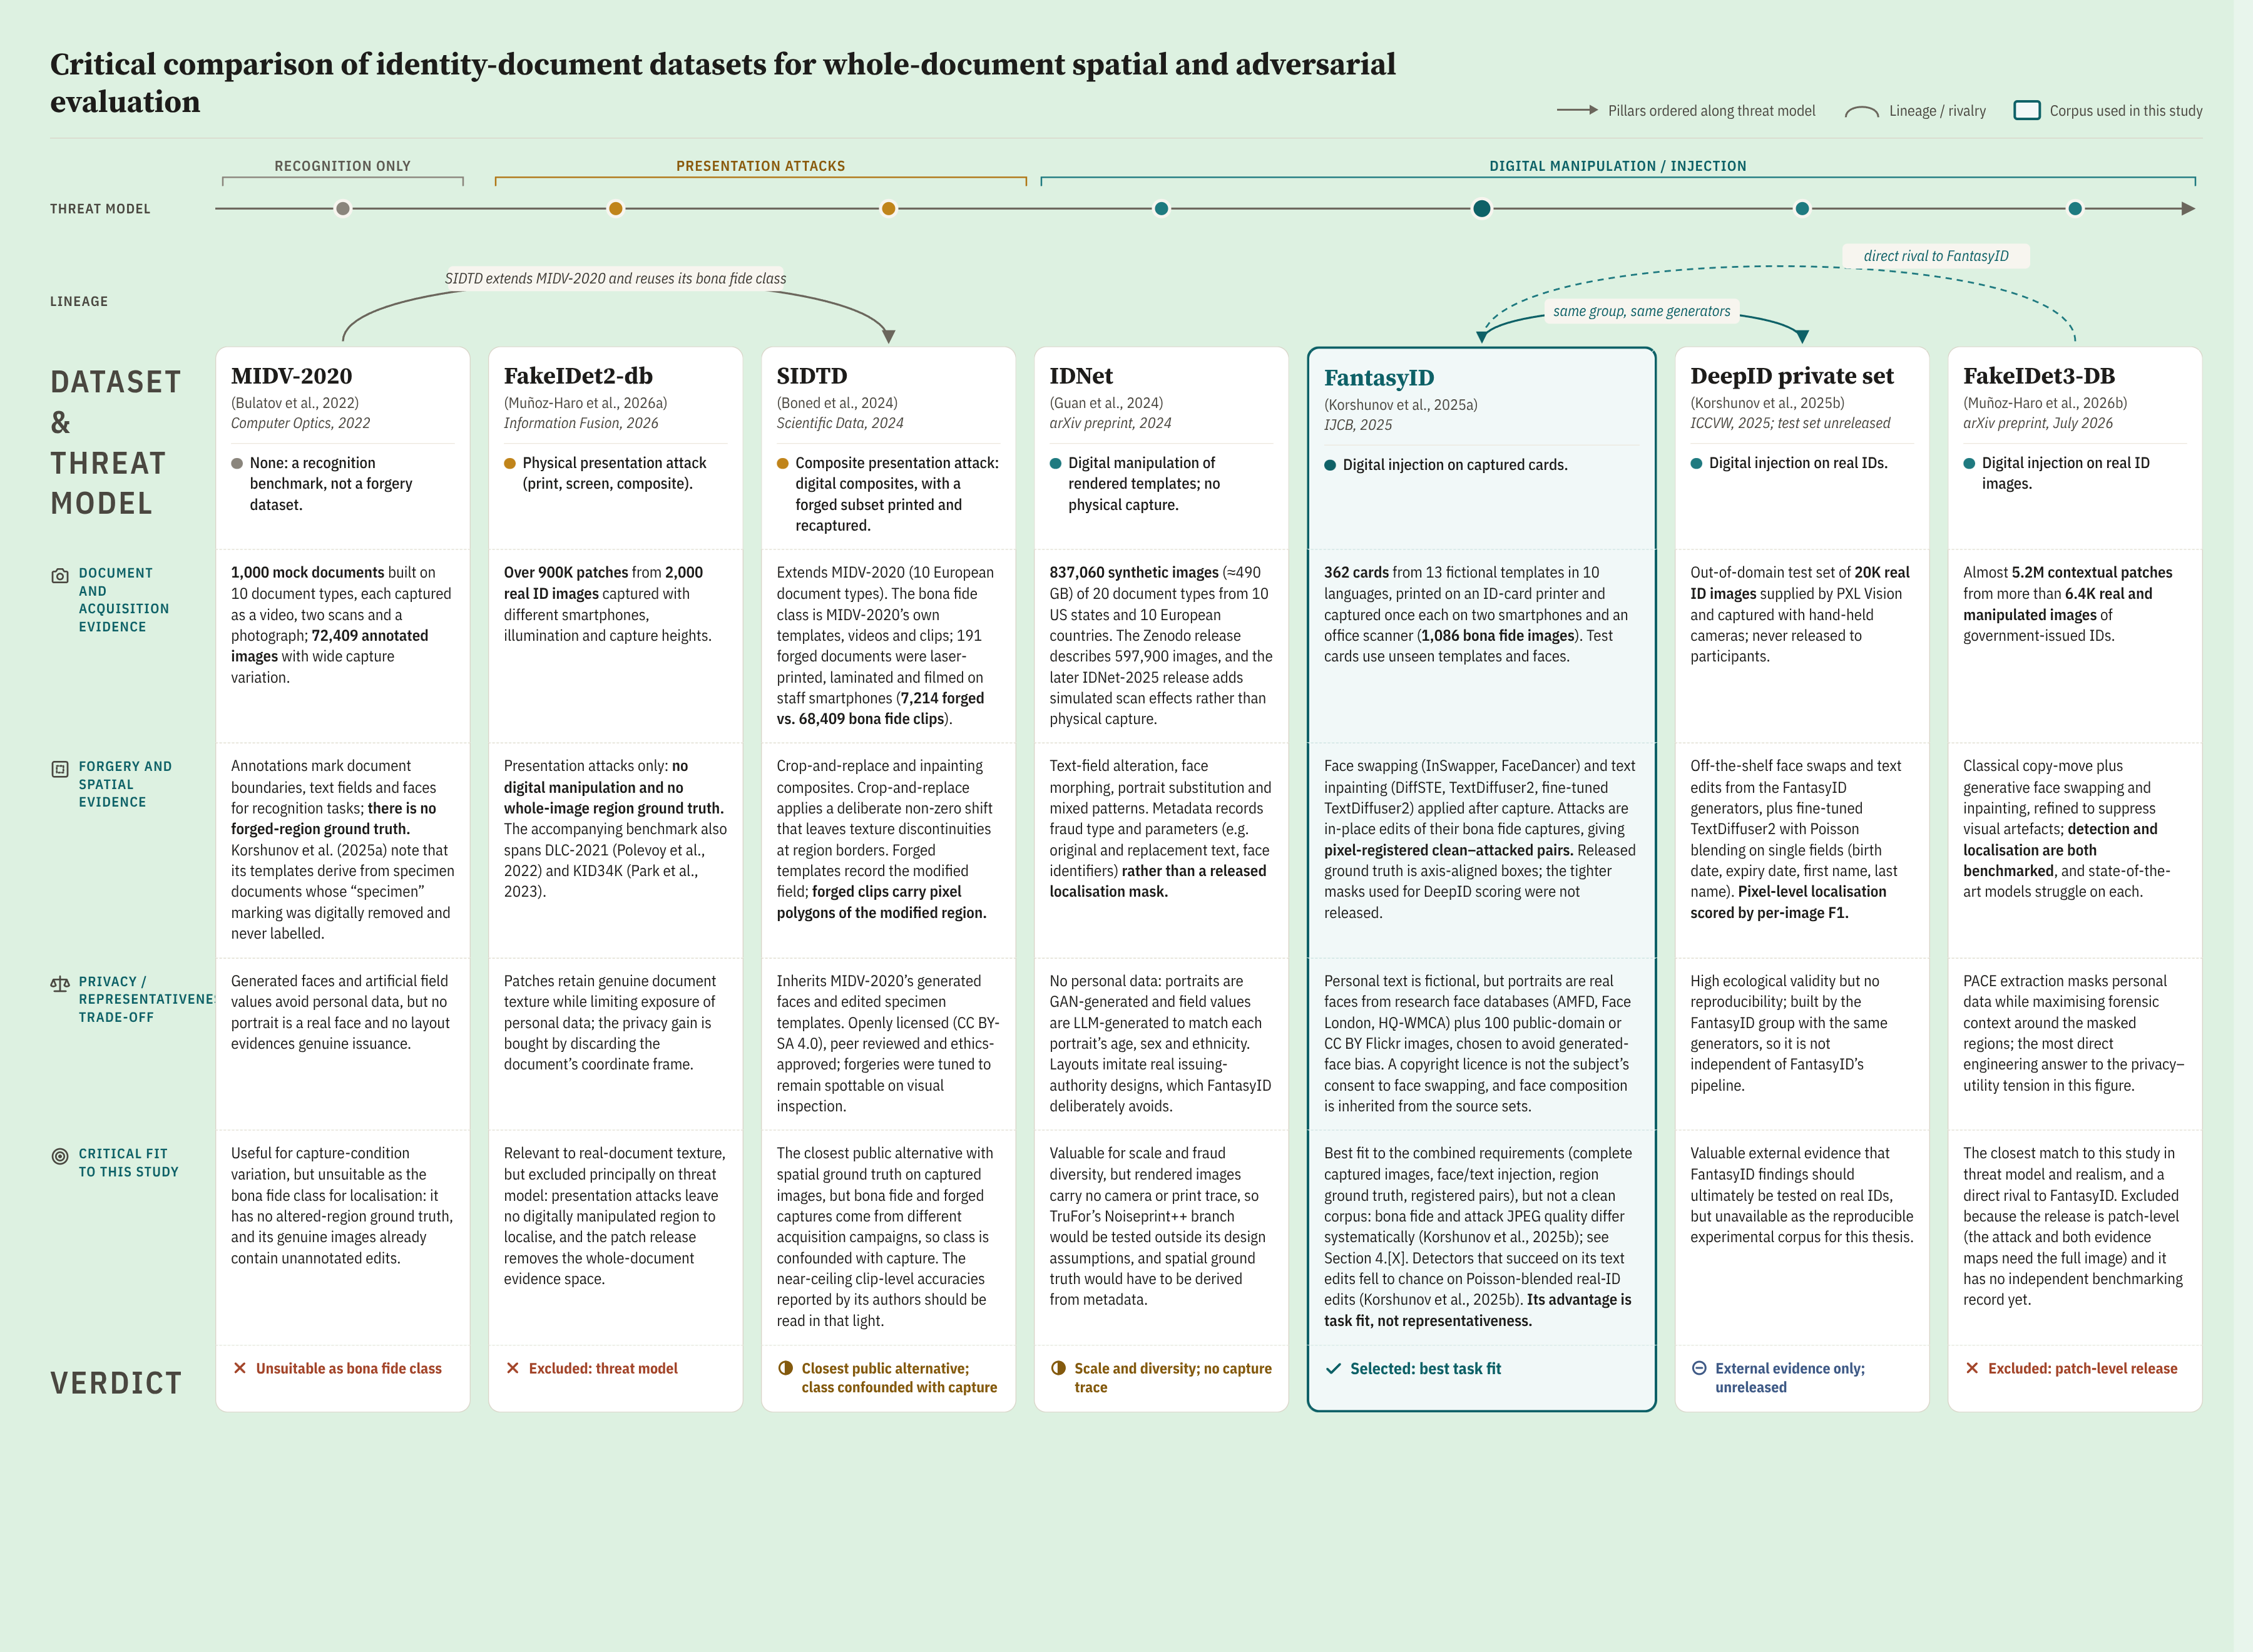
\includegraphics[
%     width=\linewidth,
%     height=0.90\textheight,
%     keepaspectratio
% ]{Images/02Dataset comparison.png}

% \vspace{0.15em}

% \captionof{table}{
% Critical comparison of ID datasets for whole-document spatial and adversarial evaluation.
% }
% \label{tab:lr-datasets}

% \end{center}

% \vfill

% \begin{center}
% \thepage
% \end{center}

% \end{landscape}

% \restoregeometry
% \clearpage
% \clearpage
% Against these requirements, publicly available identity-document datasets make different compromises. Table~\ref{tab:lr-datasets} compares the main alternatives. The comparison is task-specific and a limitation for the present ID spatial study need not be a limitation for the dataset's original purpose.

% \begin{table}[htbp]
% \centering
% \scriptsize
% \renewcommand{\arraystretch}{1.18}
% \caption{Critical comparison of ID datasets for whole-document spatial and adversarial evaluation.}
% \label{tab:lr-datasets}
% \begin{tabularx}{\textwidth}{@{}
% >{\raggedright\arraybackslash}p{0.125\textwidth}
% >{\raggedright\arraybackslash}p{0.19\textwidth}
% >{\raggedright\arraybackslash}p{0.205\textwidth}
% >{\raggedright\arraybackslash}p{0.19\textwidth}
% >{\raggedright\arraybackslash}X@{}}
% \toprule
% Dataset &
% Document and acquisition evidence &
% Forgery and spatial evidence &
% Privacy / representativeness trade-off &
% Critical fit to this study \\
% \midrule

% MIDV-2020
% \citep{bulatov2022midv2020}
% &
% 1,000 mock identity documents represented through photographs, scans and video; more than 72,000 annotated images provide substantial acquisition variation.
% &
% Designed primarily for document detection, recognition, text fields and related analysis rather than paired digital-forgery localisation. Its annotations describe document structure rather than a forged-region ground truth.
% &
% Mock documents and generated identities facilitate public research, but the source documents are artificial and are not evidence of coverage of real issuing authorities.
% &
% Strong evidence for capture-condition robustness, but it cannot directly define the altered region required for DC-DCEC-DCEW evaluation framework.
% \\

% SIDTD
% \citep{boned2024sidtd}
% &
% Extends MIDV-2020 with forged templates and printed/laminated documents captured using smartphones under varied backgrounds and illumination.
% &
% Adds crop-and-replace and inpainting attacks and provides coordinates for modified regions, making it substantially more relevant to localisation than MIDV-2020.
% &
% Retains the privacy advantages of synthetic/mock documents. However, its bona-fide source inherits the characteristics of MIDV-2020, and some crop-and-replace attacks deliberately introduce boundary discontinuities.
% &
% A credible alternative for spatial forgery research. Its manipulation construction and MIDV-derived source images differ from the injection-style face and text manipulations selected for this thesis, so success may partly reflect attack-generation artefacts rather than the intended FantasyID setting.
% \\

% IDNet
% \citep{guan2024idnet}
% &
% Large synthetic benchmark containing hundreds of thousands of identity-document images across multiple US and European document designs.
% &
% Includes text-field replacement, face morphing, portrait substitution and mixed fraud patterns, giving broader semantic fraud coverage than recognition-only datasets.
% &
% Excellent scale and low privacy exposure, but document images and identities are synthetically generated. Scale therefore increases variation without reproducing the same print--capture and sensor-processing history as a photographed physical card.
% &
% Useful for studying diversity, training and cross-layout fraud patterns; less well matched to an experiment where forensic traces from physical capture and subsequent digital manipulation are part of the observed image.
% \\

% FakeIDet2-db
% \citep{munozharo2026fakeidet2}
% &
% More than 900,000 patches derived from approximately 2,000 real ID images acquired under varied smartphone, illumination and capture conditions.
% &
% Supports bona-fide and physical attacks including print, screen and composite presentation attacks; the patch formulation is designed for privacy-aware forensic modelling.
% &
% A major advantage is that patches retain texture originating from real government-issued documents while reducing disclosure of personally identifying content.
% &
% Highly relevant for real-document forensic texture, but the public patch representation removes the complete coordinate system required to ask whether a whole-document evidence map points to the actual manipulated field.
% \\

% FakeIDet3-DB
% \citep{munozharo2026fakeidet3}
% &
% Extends the privacy-aware real-ID approach to millions of contextual patches derived from thousands of real and manipulated ID images.
% &
% Includes classical copy-move and generative manipulations such as face swapping and inpainting, with both detection and localisation evaluation.
% &
% PACE-style extraction seeks to maximise contextual forensic information while suppressing personally identifying information. This directly addresses the privacy--utility tension.
% &
% Closer to the manipulation domain of this thesis than FakeIDet2, but the released representation remains patch-centred rather than a complete-document evidence space. It is also recent preprint evidence and therefore provides less mature benchmarking history.
% \\

% FantasyID
% \citep{korshunov2025fantasyid}
% &
% 362 fictional physical cards across multiple designs and languages are printed and captured using two smartphones and an office scanner, producing 1,086 bona-fide captures.
% &
% Captured images are subsequently subjected to face swapping and text inpainting, including InSwapper, FaceDancer, DiffSTE and TextDiffuser2 variants. Complete images and manipulated-region annotations allow document-level and spatial evaluation.
% &
% Avoids tampering with official government IDs and uses fictional personal information, improving reproducibility and reducing legal/privacy obstacles. It nevertheless uses publicly licensed faces of real people and only a limited set of fictional layouts and capture devices.
% &
% Best alignment with the present conjunction of requirements: complete images, physical capture history, digital face/text manipulation, region ground truth and repeatable clean--attacked comparisons. Its advantage is task fit, not superior population representativeness.
% \\

% DeepID private set
% \citep{korshunov2025deepid}
% &
% Real identity documents are used for a private evaluation set.
% &
% Includes face swapping and text manipulations of specific fields such as birth date, expiry date, first name and last name, providing stronger evidence about realistic field-level attacks.
% &
% Real-document evidence improves ecological relevance but privacy and access constraints prevent public reproduction of the benchmark.
% &
% Valuable external evidence that FantasyID findings should ultimately be tested on real IDs, but unavailable as the reproducible experimental corpus for this thesis.
% \\

% \bottomrule
% \end{tabularx}
% \end{table}

%-----------------------------------------------------------------------------------
%-----------------------------------------------------------------------------------
%-----------------------------------------------------------------------------------
% \begingroup
% \centering
% % \scriptsize
% % \renewcommand{\arraystretch}{1.18}
% \footnotesize
% \renewcommand{\arraystretch}{1.17}

% \begin{xltabular}{\textwidth}{@{}
% >{\raggedright\arraybackslash}p{0.125\textwidth}
% >{\raggedright\arraybackslash}p{0.19\textwidth}
% >{\raggedright\arraybackslash}p{0.205\textwidth}
% >{\raggedright\arraybackslash}p{0.19\textwidth}
% >{\raggedright\arraybackslash}X@{}}

% \caption{Critical comparison of ID datasets for whole-document spatial and adversarial evaluation.}
% \label{tab:lr-datasets}\\

% \toprule
% Dataset &
% Document and acquisition evidence &
% Forgery and spatial evidence &
% Privacy / representativeness trade-off &
% Critical fit to this study \\
% \midrule
% \endfirsthead

% \toprule
% Dataset &
% Document and acquisition evidence &
% Forgery and spatial evidence &
% Privacy / representativeness trade-off &
% Critical fit to this study \\
% \midrule
% \endhead

% \bottomrule
% \endfoot

% MIDV-2020
% \citep{bulatov2022midv2020}
% &
% 1,000 mock identity documents represented through photographs, scans and video; more than 72,000 annotated images provide substantial acquisition variation.
% &
% Designed primarily for document detection, recognition, text fields and related analysis rather than paired digital-forgery localisation. Its annotations describe document structure rather than a forged-region ground truth.
% &
% Mock documents and generated identities facilitate public research, but the source documents are artificial and are not evidence of coverage of real issuing authorities.
% &
% Strong evidence for capture-condition robustness, but it cannot directly define the altered region required for DC-DCEC-DCEW evaluation framework.
% \\
% \midrule

% SIDTD
% \citep{boned2024sidtd}
% &
% Extends MIDV-2020 with forged templates and printed/laminated documents captured using smartphones under varied backgrounds and illumination.
% &
% Adds crop-and-replace and inpainting attacks and provides coordinates for modified regions, making it substantially more relevant to localisation than MIDV-2020.
% &
% Retains the privacy advantages of synthetic/mock documents. However, its bona-fide source inherits the characteristics of MIDV-2020, and some crop-and-replace attacks deliberately introduce boundary discontinuities.
% &
% A credible alternative for spatial forgery research however not chosen as it inherits the limitations of MIDV-2020.
% \\
% \midrule

% IDNet
% \citep{guan2024idnet}
% &
% Large synthetic benchmark containing hundreds of thousands of identity-document images across multiple US and European document designs.
% &
% Includes text-field replacement, face morphing, portrait substitution and mixed fraud patterns, giving broader semantic fraud coverage than recognition-only datasets.
% &
% Excellent scale and low privacy exposure, but document images and identities are synthetically generated. Scale therefore increases variation without reproducing the same print--capture and sensor-processing history as a photographed physical card.
% &
% Useful for studying diversity, training and cross-layout fraud patterns; less well matched to an experiment where forensic traces from physical capture and subsequent digital manipulation are part of the observed image.
% \\
% \midrule

% FakeIDet2-db
% \citep{munozharo2026fakeidet2}
% &
% More than 900,000 patches derived from approximately 2,000 real ID images acquired under varied smartphone, illumination and capture conditions.
% &
% Supports bona-fide and physical attacks including print, screen and composite presentation attacks; the patch formulation is designed for privacy-aware forensic modelling.
% &
% A major advantage is that patches retain texture originating from real government-issued documents while reducing disclosure of personally identifying content.
% &
% Highly relevant for real-document forensic texture, but the public patch representation removes the complete coordinate system required to ask whether a whole-document evidence map points to the actual manipulated field.
% \\
% \midrule

% FakeIDet3-DB
% \citep{munozharo2026fakeidet3}
% &
% Extends the privacy-aware real-ID approach to millions of contextual patches derived from thousands of real and manipulated ID images.
% &
% Includes classical copy-move and generative manipulations such as face swapping and inpainting, with both detection and localisation evaluation.
% &
% PACE-style extraction seeks to maximise contextual forensic information while suppressing personally identifying information. This directly addresses the privacy--utility tension.
% &
% Closer to the manipulation domain of this thesis than FakeIDet2, but the released representation remains patch-centred rather than a complete-document evidence space. It is also recent preprint evidence and therefore provides less mature benchmarking history.
% \\
% \midrule

% FantasyID
% \citep{korshunov2025fantasyid}
% &
% 362 fictional physical cards across multiple designs and languages are printed and captured using two smartphones and an office scanner, producing 1,086 bona-fide captures.
% &
% Captured images are subsequently subjected to face swapping and text inpainting, including InSwapper, FaceDancer, DiffSTE and TextDiffuser2 variants. Complete images and manipulated-region annotations allow document-level and spatial evaluation.
% &
% Avoids tampering with official government IDs and uses fictional personal information, improving reproducibility and reducing legal/privacy obstacles. It nevertheless uses publicly licensed faces of real people and only a limited set of fictional layouts and capture devices.
% &
% Best alignment with the present conjunction of requirements: complete images, physical capture history, digital face/text manipulation, region ground truth and repeatable clean--attacked comparisons. Its advantage is task fit, not superior population representativeness.
% \\
% \midrule

% DeepID private set
% \citep{korshunov2025deepid}
% &
% Real identity documents are used for a private evaluation set.
% &
% Includes face swapping and text manipulations of specific fields such as birth date, expiry date, first name and last name, providing stronger evidence about realistic field-level attacks.
% &
% Real-document evidence improves ecological relevance but privacy and access constraints prevent public reproduction of the benchmark.
% &
% Valuable external evidence that FantasyID findings should ultimately be tested on real IDs, but unavailable as the reproducible experimental corpus for this thesis.
% \\

% \bottomrule
% \end{xltabular}

% \endgroup

%---------------------------------------------

% % \begin{figure}[htbp]
% % \centering
% % \includegraphics[width=0.96\textwidth]{Images/CH02_MassRank_V1.pdf}
% % \caption{Same relevance mass, different rank overlap. Both illustrative maps put 80\% of their mass inside the annotation; one and four of their strongest four pixels fall there, respectively. These are constructed examples, not experimental results.}
% % \label{fig:lr-mass-rank}
% % \end{figure}

% Critical comparison of ID datasets (revised September 2026)
% Requires: booktabs, xltabular, array, natbib, cleveref
% Replace sec:evidence-audit with the label of your Chapter 4 evidence-audit section.
%%%%%%%%%%%%%%%%%%%%%%%%%%SAREVIEW-TABLE-TO-DIAGRAM
% \begingroup
% \centering
% \footnotesize
% \renewcommand{\arraystretch}{1.15}
% \setlength{\tabcolsep}{3.5pt}

% \begin{xltabular}{\textwidth}{@{}
% >{\raggedright\arraybackslash}p{0.105\textwidth}
% >{\raggedright\arraybackslash}p{0.10\textwidth}
% >{\raggedright\arraybackslash}p{0.175\textwidth}
% >{\raggedright\arraybackslash}p{0.19\textwidth}
% >{\raggedright\arraybackslash}p{0.17\textwidth}
% >{\raggedright\arraybackslash}X@{}}

% \caption{Critical comparison of identity-document datasets for whole-document spatial and adversarial evaluation. The line under each dataset name gives its publication status at the time of writing (September 2026).}
% \label{tab:lr-datasets}\\

% \toprule
% Dataset &
% Threat model &
% Document and acquisition evidence &
% Forgery and spatial evidence &
% Privacy / representativeness trade-off &
% Critical fit to this study \\
% \midrule
% \endfirsthead

% \toprule
% Dataset &
% Threat model &
% Document and acquisition evidence &
% Forgery and spatial evidence &
% Privacy / representativeness trade-off &
% Critical fit to this study \\
% \midrule
% \endhead

% \bottomrule
% \endfoot

% MIDV-2020
% \citep{bulatov2022midv2020}
% \newline\textit{Computer Optics, 2022}
% &
% None: a recognition benchmark, not a forgery dataset.
% &
% 1,000 mock documents built on 10 document types, each captured as a video, two scans and a photograph; 72,409 annotated images with wide capture variation.
% &
% Annotations mark document boundaries, text fields and faces for recognition tasks; there is no forged-region ground truth. \citet{korshunov2025fantasyid} note that its templates derive from specimen documents whose ``specimen'' marking was digitally removed and never labelled.
% &
% Generated faces and artificial field values avoid personal data, but no portrait is a real face and no layout evidences genuine issuance.
% &
% Useful for capture-condition variation, but unsuitable as the bona-fide class for localisation: it has no altered-region ground truth, and its genuine images already contain unannotated edits.
% \\
% \midrule

% SIDTD
% \citep{boned2024sidtd}
% \newline\textit{Scientific Data, 2024}
% &
% Composite presentation attack: digital composites, with a forged subset printed and recaptured.
% &
% Extends MIDV-2020 (10 European document types). The bona-fide class is MIDV-2020's own templates, videos and clips; 191 forged documents were laser-printed, laminated and filmed on staff smartphones (7,214 forged vs.\ 68,409 bona-fide clips).
% &
% Crop-and-replace and inpainting composites. Crop-and-replace applies a deliberate non-zero shift that leaves texture discontinuities at region borders. Forged templates record the modified field; forged clips carry pixel polygons of the modified region.
% &
% Inherits MIDV-2020's generated faces and edited specimen templates. Openly licensed (CC BY-SA 4.0), peer reviewed and ethics-approved; forgeries were tuned to remain spottable on visual inspection.
% &
% The closest public alternative with spatial ground truth on captured images, but bona-fide and forged captures come from different acquisition campaigns, so class is confounded with capture. The near-ceiling clip-level accuracies reported by its authors should be read in that light.
% \\
% \midrule

% IDNet
% \citep{guan2024idnet}
% \newline\textit{arXiv preprint, 2024}
% &
% Digital manipulation of rendered templates; no physical capture.
% &
% 837,060 synthetic images ($\approx$490\,GB) of 20 document types from 10 US states and 10 European countries. The Zenodo release describes 597,900 images, and the later IDNet-2025 release adds simulated scan effects rather than physical capture.
% &
% Text-field alteration, face morphing, portrait substitution and mixed patterns. Metadata records fraud type and parameters (e.g.\ original and replacement text, face identifiers) rather than a released localisation mask.
% &
% No personal data: portraits are GAN-generated and field values are LLM-generated to match each portrait's age, sex and ethnicity. Layouts imitate real issuing-authority designs, which FantasyID deliberately avoids.
% &
% Valuable for scale and fraud diversity, but rendered images carry no camera or print trace, so TruFor's Noiseprint++ branch would be tested outside its design assumptions, and spatial ground truth would have to be derived from metadata.
% \\
% \midrule

% FakeIDet2-db
% \citep{munozharo2026fakeidet2}
% \newline\textit{Information Fusion, 2026}
% &
% Physical presentation attack (print, screen, composite).
% &
% Over 900K patches from 2,000 real ID images captured with different smartphones, illumination and capture heights.
% &
% Presentation attacks only: no digital manipulation and no whole-image region ground truth. The accompanying benchmark also spans DLC-2021 \citep{polevoy2022dlc2021} and KID34K \citep{park2023kid34k}.
% &
% Patches retain genuine document texture while limiting exposure of personal data; the privacy gain is bought by discarding the document's coordinate frame.
% &
% Relevant to real-document texture, but excluded principally on threat model: presentation attacks leave no digitally manipulated region to localise, and the patch release removes the whole-document evidence space.
% \\
% \midrule

% FakeIDet3-DB
% \citep{munozharo2026fakeidet3}
% \newline\textit{arXiv preprint, July 2026}
% &
% Digital injection on real ID images.
% &
% Almost 5.2M contextual patches from more than 6.4K real and manipulated images of government-issued IDs.
% &
% Classical copy-move plus generative face swapping and inpainting, refined to suppress visual artefacts; detection and localisation are both benchmarked, and state-of-the-art models struggle on each.
% &
% PACE extraction masks personal data while maximising forensic context around the masked regions; the most direct engineering answer to the privacy--utility tension in this table.
% &
% The closest match to this study in threat model and realism, and a direct rival to FantasyID. Excluded because the release is patch-level (the attack and both evidence maps need the full image) and it has no independent benchmarking record yet.
% \\
% \midrule

% FantasyID
% \citep{korshunov2025fantasyid}
% \newline\textit{IJCB, 2025}
% &
% Digital injection on captured cards.
% &
% 362 cards from 13 fictional templates in 10 languages, printed on an ID-card printer and captured once each on two smartphones and an office scanner (1,086 bona-fide images). Test cards use unseen templates and faces.
% &
% Face swapping (InSwapper, FaceDancer) and text inpainting (DiffSTE, TextDiffuser2, fine-tuned TextDiffuser2) applied after capture. Attacks are in-place edits of their bona-fide captures, giving pixel-registered clean--attacked pairs. Released ground truth is axis-aligned boxes; the tighter masks used for DeepID scoring were not released.
% &
% Personal text is fictional, but portraits are real faces from research face databases (AMFD, Face London, HQ-WMCA) plus 100 public-domain or CC~BY Flickr images, chosen to avoid generated-face bias. A copyright licence is not the subject's consent to face swapping, and face composition is inherited from the source sets.
% &
% Best fit to the combined requirements (complete captured images, face/text injection, region ground truth, registered pairs), but not a clean corpus: bona-fide and attack JPEG quality differ systematically \citep{korshunov2025deepid}; see \cref{sec:evidence-audit}. Detectors that succeed on its text edits fell to chance on Poisson-blended real-ID edits \citep{korshunov2025deepid}. Its advantage is task fit, not representativeness.
% \\
% \midrule

% DeepID private set
% \citep{korshunov2025deepid}
% \newline\textit{ICCVW, 2025; test set unreleased}
% &
% Digital injection on real IDs.
% &
% Out-of-domain test set of 20K real ID images supplied by PXL Vision and captured with hand-held cameras; never released to participants.
% &
% Off-the-shelf face swaps and text edits from the FantasyID generators, plus fine-tuned TextDiffuser2 with Poisson blending on single fields (birth date, expiry date, first name, last name). Pixel-level localisation scored by per-image F1.
% &
% High ecological validity but no reproducibility; built by the FantasyID group with the same generators, so it is not independent of FantasyID's pipeline.
% &
% Valuable external evidence that FantasyID findings should ultimately be tested on real IDs, but unavailable as the reproducible experimental corpus for this thesis.
% \\

% \end{xltabular}

% \endgroup

%--------------------saREVIEW-ENDS----------------------------------

%----------------------------------------------

% Scope paragraph for the body text, placed after Table~\ref{tab:lr-datasets}.
%<sareview>
% Three further groups of datasets were excluded before comparison. 
% \begin{itemize}
%     \item Presentation-attack corpora such as DLC-2021 \citep{polevoy2022dlc2021} and KID34K \citep{park2023kid34k}, together with the private data of the PAD-ID card competitions \citep{tapia2024padid,tapia2025padid2}, address recapture rather than digital manipulation and therefore offer no manipulated region to localise.
%     \item BID \citep{soares2020bid} and FMIDV \citep{alghadi2023fmidv} are unsuitable because their bona-fide images are themselves digitally altered: BID replaces the personal details on real Brazilian identity cards, and FMIDV applies copy-move operations to MIDV-2020 images \citep{korshunov2025fantasyid}.
    
%     \item Finally, the proprietary FREUID dataset \citep{freuid2026}, released under a non-commercial licence for the IJCAI-ECAI 2026 challenge, prints and recaptures digital forgeries across seven Asian and African document types, on the argument that detectors trained on purely digital forgeries rely on artefacts that print-and-capture removes. Its published protocol scores detection only, so it provides no localisation benchmark for this study.
% \end{itemize}


No dataset dominates all of these criteria. A recurring trade-off is visible between \emph{forensic realism} and \emph{privacy-preserving reproducibility}. 

% MIDV-2020 and IDNet make broad public experimentation possible through artificial identities, but their synthetic origins limit the conclusions that can be drawn about real document capture traces. FakeIDet2 and FakeIDet3 move in the opposite direction: they expose forensic texture from real documents while withholding the complete document through privacy-aware patch extraction. This is advantageous for privacy-preserving detector development but conflicts with the present requirement to compare a whole-document spatial map with a known altered region.

% SIDTD sits between these positions. It combines physical recapture with explicitly generated forgeries and modified-region coordinates, making it a meaningful alternative for spatial research \citep{boned2024sidtd}. However, its bona-fide images derive from MIDV-2020 and its crop-and-replace procedure can introduce boundary discontinuities by design. For the present research question, this creates a possible shortcut: a model may learn generation-specific artefacts rather than evidence associated with the manipulated semantic field. This does not invalidate SIDTD, but makes its threat model different from the digital injection setting investigated here.

FantasyID provides the closest conjunction of the required properties. Its fictional cards are physically printed and recaptured before digital manipulation, so the forged samples retain a physical acquisition history while face and text regions are subsequently altered using contemporary generative tools \citep{korshunov2025fantasyid}. It also preserves the complete image and known alteration regions. These properties permit the same forged image to be assessed for the DC-DCEC-DCEW framework of this study.

These strengths come with two cautions from its authors' later work. bona-fide and attacked images differ systematically in JPEG quality, a shortcut a detector can exploit without examining the edited field, which is why Chapter~3 controls compression before training. In the DeepID challenge, detectors that performed well on FantasyID's text edits fell to chance on Poisson-blended edits of real IDs \citep{korshunov2025deepid}. Because DeepID shares FantasyID's authors and generators, this is the strongest available transfer warning rather than independent validation.

% at three levels required by this thesis: whether the detector makes the correct forgery decision, whether its clean spatial evidence agrees with the altered region, and whether an adversary can subsequently degrade that spatial evidence while preserving the decision.

% This selection should not be interpreted as evidence that FantasyID is representative of operational identity verification as a whole. NIST AI RMF and the representativeness principles reflected in the EU AI Act instead expose its principal limitations: a small set of fictional layouts cannot represent the document designs of real issuing authorities, three capture devices cannot span deployment conditions, and repeated captures of the same physical card are not independent observations \citep{nist2023airmf,eu2024aiact}. The dataset is therefore selected for \emph{experimental identifiability and reproducibility}, not for regulatory validation or population-level deployment claims.

% The DeepID challenge provides an important external check on this distinction. Its private evaluation uses real identity documents and includes field-specific face and text manipulations that cannot be reproduced from the public FantasyID corpus \citep{korshunov2025deepid}. The challenge also reports that a participating team observed different JPEG quality factors between bona-fide and manipulated samples. Such a difference is important because a detector could obtain the correct label from processing history rather than from the altered field. The present study therefore does not assume that correct classification establishes forensic validity. A compression-control audit is conducted before spatial eligibility is interpreted.

% Finally, three dataset-specific dependencies are carried forward into the experimental design. First, the available alteration annotations are approximations of the manipulated region rather than perfect semantic ground truth; spatial conclusions therefore require sensitivity checks and more than one measure of agreement. Second, multiple captures derived from the same underlying physical card are dependent observations, so uncertainty estimates and data partitions must respect document stem. Third, fictional documents cannot establish performance across real issuing authorities, nationalities or operational KYC systems. These limitations motivate the mask-sensitivity checks, stem-grouped analysis and restricted external-validity claims defined in Chapter~3 and reported in the subsequent experimental chapters.

Three limitations or risks remain after dataset selection:
\begin{enumerate}
    \item Rectangular annotations approximate the altered regions
    \item Capture variants of one card are dependent observations
    \item Fictional documents cannot establish performance across real issuing authorities.
\end{enumerate}

These motivate mitigating strategies including mask-sensitivity checks, grouping by document stem and restricted claims. Chapter~3 defines these controls, Appendix~A records metric-related risks and the model-specific registers retain preprocessing decisions.

%--------------------------------------------------------------------------------------------------
% \section{Two routes to spatial evidence}
% \label{sec:lr-where}

% \subsection{Post-hoc attribution and ResNet-18 with Grad-CAM}

% Grad-CAM uses gradients of a target score to weight convolutional feature maps, producing a regional indication of class evidence \citep{selvaraju2017gradcam}. It can be applied after classifier training. ResNet-18 supplies an established residual classifier that is manageable for repeated training and attacks \citep{he2016resnet}. This makes the combination a suitable experimental representative without making architecture development part of the research question.

% Other attribution methods offer different trade-offs. Integrated Gradients attributes a prediction relative to a reference input and satisfies explicit sensitivity and implementation-invariance axioms \citep{sundararajan2017axiomatic}. Score-CAM weights activation maps using forward-pass scores instead of gradients \citep{wang2020scorecam}. Neither turns classifier attribution into a supervised forgery mask. Grad-CAM is retained for a focused study of an established method; its selection does not imply that it is the most faithful explainer.

% The explanation target also matters. Finer-CAM contrasts a target class with a reference class to suppress shared features \citep{zhang2025finercam}. This supports explaining the manipulated-minus-bona-fide score difference in a binary classifier. It provides a rationale for that target, not evidence that it will localise document alterations successfully. The exact target and layer belong in Chapter~3 and Appendix~B.

% A coarse feature grid places a further limit on interpretation. Enlarging its map does not restore missing character-level detail. Moreover, a classifier may correctly detect global compression differences, so an attribution outside the edited region need not be an inaccurate account of its behaviour. Clean spatial agreement therefore requires separate assessment before any loss is attributed to an attack.

% \subsection{Native localisation and TruFor}

% TruFor combines RGB information with Noiseprint++, a learned representation of processing traces. Its transformer-based fusion produces a manipulation map and a confidence map; pooled statistics from these maps feed the image-level decision \citep{guillaro2023trufor}. Unlike Grad-CAM, its manipulation output is explicitly trained for localisation. The connection between map and decision makes decision-preserving degradation worth testing, but does not guarantee that one must fail whenever the other fails.

% TruFor has direct precedent as a DeepID baseline. The challenge also demonstrates document-specific adaptation of pretrained forensic models \citep{korshunov2025deepid}. EdgeDoc provides another example of combining forensic traces and visual features for identity documents \citep{george2025edgedoc}. These developments support studying native localisation, while showing that pipeline performance depends on training and adaptation as well as architecture.

% This thesis retains pretrained TruFor as a native baseline. Any fine-tuned condition requires its own clean evaluation; improvement is an empirical question. Training ResNet-18 on documents and using pretrained TruFor does not equalise domain exposure, and fine-tuning both would not equalise their supervision or pretraining. Each pipeline is therefore assessed against its own clean evidence. Shared eligible images provide an additional view, not a basis for attributing differences to architecture alone.


\section{Two routes to spatial evidence}
\label{sec:lr-where}

\subsection{Post-hoc attribution and ResNet-18 with Grad-CAM}

Grad-CAM uses gradients of a target score to weight convolutional feature maps, producing a coarse class-discriminative localisation map \citep{selvaraju2017gradcam}. Because it is applied after classifier training, localisation supervision is not required. ResNet-18 provides an established residual classifier that remains tractable for repeated training and adversarial optimisation \citep{he2016resnet}. The combination therefore provides a conventional classifier--attribution pipeline without making architecture development part of the research question.

Alternative attribution methods represent different design choices. Integrated Gradients is a path-based attribution method that explains a prediction relative to a reference input and satisfies Sensitivity and Implementation Invariance, although its result depends on the baseline \citep{sundararajan2017axiomatic}. Score-CAM represents a forward-pass, perturbation-style CAM alternative that avoids gradient-based weighting but increases computational cost when explanations must be generated repeatedly \citep{wang2020scorecam}. Finer-CAM addresses a different choice namely ``the explanation target'', by contrasting a target class with a reference class to suppress shared features \citep{zhang2025finercam}. None of these alternatives converts classifier attribution into a supervised forgery mask. Grad-CAM is therefore retained as an established and computationally suitable representative, not as a claim that it is the most faithful attribution method.

% Alternative attribution methods change what is gained and what is assumed. Integrated Gradients attributes a prediction relative to a reference input and satisfies Sensitivity and Implementation Invariance, but its result depends on the choice of baseline \citep{sundararajan2017axiomatic}. Score-CAM avoids gradient-based weighting by measuring activation-map contributions through forward passes \citep{wang2020scorecam}; this removes one dependence on gradients but increases computational cost when explanations must be generated repeatedly. Neither method converts classifier attribution into a supervised forgery mask. Grad-CAM is therefore retained as an established and computationally suitable representative, not as a claim that it is the most faithful attribution method.

Finer-CAM does also show that contrasting a target class against a reference class can suppress features shared between classes and expose finer discriminative cues \citep{zhang2025finercam}. This motivates a contrastive manipulated-versus-bona-fide target in the binary classifier, but does not establish that such a map will coincide with the document alteration. The exact target and layer are therefore methodological choices defined in Chapter~3 and Appendix~B.

Spatial resolution imposes a separate limitation. Upsampling a coarse convolutional map cannot recover character-level information absent from its feature grid. More importantly, disagreement with the manipulation mask is not automatically evidence that Grad-CAM inaccurately represents the classifier: a correct decision may genuinely depend on compression or other document-wide cues. Clean spatial agreement must therefore be established separately before adversarial degradation is interpreted.

\subsection{Native localisation and TruFor}

TruFor approaches the problem differently. It combines RGB features with Noiseprint++, a learned representation of camera and processing traces, through transformer-based fusion \citep{guillaro2023trufor}. It produces an anomaly map and an associated confidence map; confidence-weighted pooling summarises these outputs before a classifier produces the image-level integrity score. Unlike Grad-CAM, localisation is therefore an explicitly trained component of the forensic pipeline. This structural connection makes decision-preserving spatial degradation a stronger constraint, while still leaving open whether substantial map changes can occur without changing the final decision.

% TruFor is not the only native-localisation alternative. DeepID used it as a baseline and showed that document-specific adaptation of forensic models can improve performance \citep{korshunov2025deepid}. EdgeDoc goes further by combining a lightweight visual transformer with noiseprint features specifically for identity-document forgery detection and localisation \citep{george2025edgedoc}. Such systems may be better adapted to this domain, but using them would also introduce additional task-specific training and supervision into the comparison.

Similar to post-hoc attribution, Native localisation also has alternatives offering different design choices. TruFor represents a general-purpose forensic model with explicit manipulation localisation, while DeepID demonstrates document-specific adaptation of pretrained forensic models \citep{korshunov2025deepid}. EdgeDoc represents a more directly domain-adapted alternative by combining visual and forensic-trace features specifically for identity-document forgery detection and localisation \citep{george2025edgedoc}. Such systems may benefit from task-specific training, but adopting them would also change the amount and type of domain supervision in the comparison. TruFor is therefore retained as a pretrained native-localisation baseline rather than as the strongest possible document-specific model.

A document-trained ResNet-18 and pretrained TruFor do not have equal domain exposure, but fine-tuning both would not equalise their objectives, pretraining or supervision either. Architecture-level ranking would consequently be misleading. Each pipeline is evaluated against its own clean evidence, while results on shared eligible images provide a controlled supplementary comparison rather than evidence that one architecture is intrinsically superior.



% \section{What should count as acceptable spatial evidence?}
% \label{sec:lr-metrics}

% \subsection{Spatial agreement and explanation faithfulness}

% A visually convincing map can be misleading. Randomisation tests show that some saliency methods retain structure after learned model information is disrupted \citep{adebayo2018sanity}. Such tests assess dependence on the model; annotation overlap asks a different question. A map may reflect a classifier's reliance on a shortcut accurately while offering little help in finding the alteration. Here, ``evidence correct'' means meeting a declared spatial-agreement criterion. It is not a general certificate of explanation quality.

% Pixel-F1 and intersection-over-union are appropriate for evaluating predicted segmentation masks. TruFor reports F1 with a fixed threshold and with the best threshold for each image \citep{guillaro2023trufor}. The latter uses ground truth unavailable during deployment. Applying an arbitrary probability threshold to Grad-CAM is also problematic because its values are relative attribution strengths. F1 and IoU remain useful localisation diagnostics, but a common primary criterion should accommodate both kinds of continuous map.

% \subsection{Relevance mass and relevance rank}

% Score-CAM evaluates how much saliency energy falls inside an annotated region \citep{wang2020scorecam}. CLEVR-XAI defines relevance mass accuracy and relevance rank accuracy for evaluating non-negative explanation maps against ground truth \citep{arras2022clevrxai}. These provide the literature basis for the two quantities used here.

% Let $S(p)$ be the non-negative spatial value at pixel $p$, $M$ the union of annotated manipulation regions, and $\Omega$ the valid document area. With $K=|M|$, the measures are
% \begin{equation}
% E=\frac{\sum_{p\in M}S(p)}{\sum_{p\in\Omega}S(p)},
% \qquad
% \mathrm{RRA}=\frac{|\operatorname{TopK}_{K}(S)\cap M|}{K}.
% \label{eq:lr-mass-rank}
% \end{equation}
% The top-$K$ pixels are selected within $\Omega$. Both measures range from zero to one for valid maps and non-empty masks.

% $E$ asks how much of the map's total mass lies inside the annotation. RRA asks how many of its strongest pixels fall there when the selected set has the same area as the annotation. Figure~\ref{fig:lr-mass-rank} shows why these questions differ: identical mass containment can accompany very different rank overlap. RRA adds a check on the spatial distribution of strong evidence, although it does not prove that every altered feature has been identified.

% %<sareview>
% % \begin{figure}[htbp]
% % \centering
% % \includegraphics[width=0.96\textwidth]{Images/CH02_MassRank_V1.pdf}
% % \caption{Same relevance mass, different rank overlap. Both illustrative maps put 80\% of their mass inside the annotation; one and four of their strongest four pixels fall there, respectively. These are constructed examples, not experimental results.}
% % \label{fig:lr-mass-rank}
% % \end{figure}

% The transfer from CLEVR-XAI needs qualification. Its controlled visual-question-answering setting can identify relevant objects by construction. An identity-document annotation identifies an edited region, which need not contain every cue used by a forgery classifier. Applying the measures to TruFor also evaluates the distribution of manipulation scores, rather than classifier relevance. The equations provide common spatial measurements without making the maps equivalent explanations.

% \subsection{Why two measures still need supporting checks}

% Neither measure removes region-size effects. If $A=|M|/|\Omega|$, a uniform map gives $E=A$. The area-normalised quantity $\mu_w=E/A$ is consequently useful as a diagnostic, but can be large when little total evidence lies inside a small region. For example, $A=0.01$ and $E=0.02$ give $\mu_w=2$, although 98\% of the mass remains outside. A mass requirement is therefore still needed.

% RRA also depends on annotation size and geometry. Under spatially random ranking its expected value is $A$; its top-$K$ boundary can be sensitive to tied values. Both measures are unchanged by multiplying a valid map by a positive constant, so they describe spatial allocation rather than absolute confidence. Zero or invalid maps need explicit handling, not arbitrary normalisation. Interpolation, padding and broad rectangles can further affect both scores.

% The Pointing Game checks whether the strongest location falls inside the target region \citep{zhang2016excitation}. It is easy to interpret, but one successful pixel cannot establish regional agreement. PG, $A$, $\mu_w$ and face/text measurements therefore remain supporting diagnostics. A union mask can also hide uneven performance: a large portrait region may dominate while a small text edit receives little evidence. Component-level measurements and visual examples help expose this limitation. Chapter~4 also retains continuous $E$ and RRA values: averages alone cannot identify which individual images satisfy both requirements.

% The literature supplies these measures, but does not establish a universal threshold for acceptable evidence in this task. This study combines $E\geq\tau_E$ and $\mathrm{RRA}\geq\tau_{\mathrm{RRA}}$. The thresholds require calibration from clean development data, supported by visual judgements made without seeing the numerical metrics. The same procedure applies to both pipelines, while numerical thresholds may differ. Chapter~3 specifies selection and freezing; Appendix~A records the rating scheme, alternatives, tie handling, boundary sensitivity and calibration uncertainty. A visual judgement remains a fallible reference, and calibration agreement is not independent validation.

%%%%%%%%%%%%%%%%%%%%%%%%%%%%%%%%version 02 %%%%%%%%%%%%%%%%%%%%%%%%%%%%%%%%%%%%%%%%%%

% \section{What should count as acceptable spatial evidence?}
% \label{sec:lr-metrics}

% \subsection{Spatial agreement is not explanation faithfulness}

% A spatial map can look convincing without reflecting what the model has learned. Randomisation tests show that some saliency methods produce near-identical maps even after the model's parameters are randomised \citep{adebayo2018sanity}. Those tests are about faithfulness to the model. Comparing a map with the manipulation mask, which marks where the forgery was made, asks a different question. It evaluates if the displayed evidence fall where the alteration occurred? The two can diverge, because a classifier may faithfully rely on compression, acquisition or other shortcut cues outside the edited field. For this reason, ``acceptable spatial evidence'' therefore means meeting a declared spatial-agreement rule, not providing a complete or causally faithful explanation.

% Standard segmentation measures, the obvious candidates, are also an awkward common gate. Pixel-F1 and intersection-over-union suit binary regions, and TruFor reports F1 at both a fixed threshold and the best per-image threshold \citep{guillaro2023trufor}. \citep{guillaro2023trufor}. The second is chosen using ground truth, which no deployed system has, introducing a significant validation pitfall where test-stage optimization overestimates real-world utility \citep{maier2024metrics}. Grad-CAM, meanwhile, gives relative attribution strengths, not calibrated manipulation probabilities, so one numerical threshold would mean different things in each pipeline. F1 and IoU remain useful diagnostics, but the primary criterion should compare continuous, non-negative maps without binarising them first.

% \subsection{Why relevance mass and relevance rank are combined}

% Score-CAM motivates measuring the proportion of saliency energy inside a target region \citep{wang2020scorecam}, while CLEVR-XAI formalises complementary relevance mass accuracy(RMA) and relevance rank accuracy(RRA) for non-negative maps \citep{arras2022clevrxai}. Let $S(p)$ be the spatial value at pixel $p$, $M$ the union of annotated manipulation regions, $\Omega$ the valid document area, and $K=|M|$:
% \begin{equation}
% E=\frac{\sum_{p\in M}S(p)}{\sum_{p\in\Omega}S(p)},
% \qquad
% \mathrm{RRA}=\frac{|\operatorname{TopK}_{K}(S)\cap M|}{K}.
% \label{eq:lr-mass-rank}
% \end{equation}

% The two measures address different failure modes. 
% \begin{itemize} [itemsep=1pt]
%     \item $E$ asks how much total map mass lies inside the alteration, but does not require the strongest responses to be concentrated there.
%     \item RRA asks whether the highest-ranked pixels occupy the alteration, but ranking alone does not ensure that it receives a substantial share of total evidence.
% \end{itemize}
% Their conjunction is therefore more defensible than either measure alone. This motivates DCEC: among samples already satisfying decision correctness (DC), clean evidence is accepted only when both $E\geq\tau_E$ and $\mathrm{RRA}\geq\tau_{\mathrm{RRA}}$.

% The transfer from CLEVR-XAI still needs qualification for this study. Its relevant objects can be specified by construction because an ID-document mask marks edited pixels, not necessarily every cue legitimately used by a forgery detector. 
% The equations also have different semantics across pipelines: 
% \begin{itemize} [itemsep=0pt]
%     \item For Grad-CAM, they measure class attribution
%     \item For TruFor, they measure a learned manipulation score.
% \end{itemize}
% Hence it is clear that they provide a common test of spatial agreement, not equivalent explanations in line with the study's objective.

% \section{What should count as acceptable spatial evidence?}
% \label{sec:lr-metrics}

% \subsection{Spatial agreement is not explanation faithfulness}

% A spatial map can look convincing without reflecting what the model has learned. Randomisation tests show that some saliency methods retain substantial structure after learned model parameters are disrupted \citep{adebayo2018sanity}. Such tests concern faithfulness to the model, whereas comparison with a manipulation mask asks whether displayed evidence coincides with the known alteration. The two need not agree. A classifier may faithfully rely on compression, acquisition or other shortcut cues outside the edited field. ``Acceptable spatial evidence'' in this thesis therefore concerns spatial agreement with the manipulation rather than a claim of explanation faithfulness.

% Standard segmentation measures are also an awkward common criterion. Pixel-F1 and intersection-over-union suit binary regions, and TruFor reports F1 using both a fixed threshold and a best per-image threshold \citep{guillaro2023trufor}. The latter uses ground truth to optimise the reported result, while Grad-CAM produces relative attribution strengths rather than calibrated manipulation probabilities. Applying one numerical threshold would therefore impose different assumptions on the two pipelines. F1 and IoU remain relevant localisation measures, but continuous-map measures avoid making binarisation the primary basis of comparison.

% \subsection{Why relevance mass and relevance rank are combined}

% Score-CAM considers the proportion of saliency energy falling within an annotated region \citep{wang2020scorecam}, while CLEVR-XAI formalises relevance mass accuracy (RMA) and relevance rank accuracy (RRA) for evaluating non-negative explanation maps against ground-truth regions \citep{arras2022clevrxai}. Let $S(p)$ denote the non-negative spatial value at pixel $p$, $M$ the annotated region and $K=|M|$:
% \begin{equation}
% E=\frac{\sum_{p\in M}S(p)}{\sum_{p}S(p)},
% \qquad
% \mathrm{RRA}=\frac{|\operatorname{TopK}_{K}(S)\cap M|}{K}.
% \label{eq:lr-mass-rank}
% \end{equation}

% The measures test different properties. Relevance mass asks how much of the total spatial response lies within the target, whereas rank accuracy asks whether the strongest responses preferentially occupy it. CLEVR-XAI treats these as complementary rather than interchangeable measures \citep{arras2022clevrxai}: a map may concentrate substantial total mass inside a region without ranking its pixels most strongly, or achieve high-ranked overlap while distributing considerable mass elsewhere. For this study, that complementarity provides the literature basis for requiring both containment and concentration when defining acceptable clean spatial evidence.

% Their transfer to identity-document forgery nevertheless requires caution. CLEVR-XAI uses synthetic visual-question-answering scenes in which relevant objects can be specified by construction. A manipulation mask instead identifies where an edit occurred; it does not prove that all legitimate forensic evidence must originate there. The meaning also differs by pipeline: Grad-CAM expresses class attribution, whereas TruFor produces learned manipulation scores. RMA and RRA therefore create a common spatial comparison, not a claim that the two maps are equivalent explanations.

% \subsection{Limitations of spatial agreement metrics}

% No localisation metric is neutral to its evaluation setting. CLEVR-XAI reports changes in relevance accuracy when target-object size and prediction confidence are varied, showing that measured explanation quality also reflects properties of the evaluated sample \citep{arras2022clevrxai}. More broadly, Tomsett et al.\ show that saliency metrics can give inconsistent assessments and that implementation choices can materially affect conclusions \citep{tomsett2020sanitymetrics}. Metric choice should therefore follow the question being asked rather than assume that one score represents explanation quality generally.

% Region-based ground truth creates particular difficulties for identity documents. Large portrait alterations and very small text edits differ greatly in area, so apparent spatial agreement can partly reflect target size. Rectangular annotations may also contain unchanged pixels, while a union of several regions can conceal poor localisation of a smaller component. These effects are especially relevant where face and text manipulations coexist and argue against interpreting a single aggregate score without supporting evidence.

% Simpler alternatives illustrate the same trade-off. The Pointing Game asks only whether the maximum response lies inside the annotated region \citep{zhang2016excitation}; it is intuitive but ignores the remainder of the map, so one correctly placed peak cannot establish regional agreement. Conversely, overlap measures assess a broader region but require thresholding. The literature therefore supports using complementary spatial properties rather than treating any one localisation measure as a universal definition of acceptable evidence.

% For this thesis, these findings provide the conceptual basis for distinguishing a correct document decision (DC) from a correct decision whose clean spatial evidence is also acceptable (DCEC). The operational definition of DCEC, threshold calibration, supporting diagnostics and the subsequent decision-preserving adversarial failure condition are methodological choices and are specified in Chapter~3.


% \subsection{Calibration, baselines and supporting checks}

% Region size remains a confound. If $A=|M|/|\Omega|$, a uniform map gives $E=A$, and random ranking has expected RRA $A$. The area-normalised ratio $\mu_w=E/A$ therefore indicates enrichment above this baseline, but cannot replace $E$: a small region can obtain a large ratio while containing little total mass. The Pointing Game tests whether the strongest location lies inside the target \citep{zhang2016excitation}, but one successful pixel cannot establish regional agreement. $A$, $\mu_w$, Pointing Game, component-level face/text scores and visual examples therefore remain supporting diagnostics.

% Mask geometry and implementation also matter as they carry an inherent risk. Rectangular annotations may include unchanged pixels; a union mask can let a large portrait dominate a small text edit; ties affect the top-$K$ boundary; and interpolation, padding or invalid maps require explicit handling. Continuous $E$ and RRA values are therefore retained alongside pass/fail status.

% The literature does not provide universal thresholds for acceptable ID-document evidence. Thresholds are calibrated on clean development data with visual judgements made without access to the numerical scores, then frozen before adversarial evaluation. The procedure is common across pipelines, although numerical thresholds may differ because map semantics and distributions differ. DCEC is therefore a pipeline-specific clean eligibility condition rather than a universal quality scale, so its coverage must be reported. DCEW is counted only when an initially DCEC sample retains the correct forgery decision after attack but fails at least one frozen evidence condition. This prevents already-poor clean maps from inflating apparent adversarial vulnerability. Chapter~3 defines calibration and freezing; Appendix~A records the rating scheme and sensitivity checks.

%--------------------------------------version 03----------------------------------------------

\section{What should count as acceptable spatial evidence?}
\label{sec:lr-metrics}

\subsection{Spatial agreement is not explanation faithfulness}

A spatial map can look convincing without reflecting what the model has learned. Randomisation tests show that some saliency methods retain substantial structure after learned parameters are disrupted \citep{adebayo2018sanity}. Such tests concern faithfulness to the model; comparison with a manipulation mask asks whether displayed evidence coincides with the known alteration. The two can diverge because a classifier may faithfully rely on compression, acquisition or other shortcut cues outside the edited field. Here, ``acceptable spatial evidence'' therefore means spatial agreement with the alteration, not a general certificate of explanation faithfulness.

Standard segmentation measures are also an awkward common criterion. Pixel-F1 and intersection-over-union suit binary regions, while TruFor reports F1 using both a fixed threshold and a best per-image threshold \citep{guillaro2023trufor}. Grad-CAM instead produces relative attribution strengths rather than calibrated manipulation probabilities. A common threshold would therefore impose different assumptions on the two pipelines. F1 and IoU remain useful diagnostics, but continuous-map measures avoid making binarisation the primary basis of comparison.

\subsection{Why relevance mass and relevance rank are combined}

Score-CAM considers the proportion of saliency energy inside an annotated region \citep{wang2020scorecam}, while CLEVR-XAI formalises relevance mass accuracy (RMA), written E below and relevance rank accuracy (RRA) for non-negative maps \citep{arras2022clevrxai}. Let $S(p)$ be the spatial value at pixel $p$, $M$ the annotated manipulation region, and $K=|M|$:
\begin{equation}
E=\frac{\sum_{p\in M}S(p)}{\sum_{p}S(p)},
\qquad
\mathrm{RRA}=\frac{|\operatorname{TopK}_{K}(S)\cap M|}{K}.
\label{eq:lr-mass-rank}
\end{equation}

The measures test different properties. 
\begin{itemize}
    \item $E$ asks how much total map mass lies inside the alteration
    \item RRA asks whether the strongest responses preferentially occupy it.
\end{itemize}
A map can perform well on one while remaining weak on the other, so their combination provides a stronger basis for judging clean spatial evidence than either alone.

Their transfer from CLEVR-XAI nevertheless needs qualification. Its relevant objects are known by construction, whereas an ID-document mask marks where an edit occurred, not necessarily every cue legitimately used by a detector. 
The map semantics also differ: 
\begin{itemize}
    \item Grad-CAM expresses class attribution
    \item TruFor produces learned manipulation scores.
\end{itemize}
The measures therefore provide a common test of spatial agreement, not equivalent explanations.

\subsection{Limitations of spatial agreement metrics}

No localisation metric is independent of its evaluation setting as discussed below. 
\begin{enumerate}
    \item CLEVR-XAI reports changes in relevance accuracy with target size, while broader work shows that saliency metrics can disagree and that implementation choices can alter conclusions \citep{arras2022clevrxai,tomsett2020sanitymetrics}. This is important for identity documents, where a large portrait replacement and a small text edit differ greatly in area.
    \item Simpler alternatives have complementary weaknesses. The Pointing Game asks only whether the maximum response lies inside the target \citep{zhang2016excitation}; one successful peak cannot establish regional agreement.
    \item Conversely, overlap measures require thresholding. Rectangular or union annotations can also conceal uneven localisation across components.
\end{enumerate}

The literature therefore supports combining spatial properties rather than treating one score as a universal definition of evidence quality. These findings provide the conceptual basis for separating a correct decision (DC) from a correct decision with acceptable clean spatial evidence (DCEC). The operational definition of DCEC, threshold calibration, supporting diagnostics and the later decision-preserving adversarial failure condition are specified in Chapter~3.


%------------------------------------------------------------------------------------
% \section{Attacking explanations while preserving decisions}
% \label{sec:lr-xai-attacks}

% \citet{ghorbani2019fragile} show that small input changes can substantially alter neural-network explanations while retaining the predicted label. \citet{dombrowski2019explanations} relate this sensitivity to network geometry and steer explanations towards chosen targets while keeping outputs approximately constant. Together, these studies establish that prediction stability does not ensure explanation stability. However, a changed map is not necessarily a worse map: similarity to the clean output does not itself measure agreement with a known manipulation.

% \citet{heo2019fooling} demonstrate a different route by changing model parameters so that explanations become misleading while predictive performance is largely retained. This establishes a model-owner threat, which must be distinguished from the bounded input perturbations considered here. Combining their outcomes into one attack-success comparison would conceal differences in attacker capability.

% More recent work extends prediction-preserving manipulation to audio deepfake explanations \citep{kitlowski2026fragility}. Its study of 100 recordings supports the relevance of the failure to forensic systems, but audio-specific perceptual constraints and map-similarity measures do not answer the identity-document question. These studies motivate an adversary targeting spatial evidence and a success rule that verifies the final decision, rather than trusting a decision-preservation term in the optimisation loss.


\section{Attacking spatial evidence while preserving forgery decisions}
\label{sec:lr-xai-attacks}

\citet{ghorbani2019fragile} show that small input perturbations can alter attribution maps while preserving the predicted label. \citet{dombrowski2019explanations} steer explanations towards chosen targets and relate the effect to network geometry. Together they establish the separation used here: prediction stability does not imply spatial-evidence stability. Their experiments concern generic image classification and mainly measure departure from the clean explanation. 
% % In identity documents, however, the manipulation region is known and may range from a few characters to an entire portrait; degradation can therefore be judged against the forgery while the document remains correctly classified as forged.
% In the controlled benchmark setting used here, the manipulated region is known from dataset annotations and may range from a few altered characters to an entire portrait. This makes it possible to evaluate whether an attack moves spatial evidence away from the true edit while the document is still correctly classified as forged; such ground truth would not ordinarily be available during deployment.

In the controlled benchmark setting used here, dataset annotations identify the true manipulated region, which may range from a few characters to an entire portrait. This allows spatial degradation to be measured against the actual edit while the forgery decision is preserved, even though such ground truth is unavailable in deployment.

\citet{heo2019fooling} instead modify model parameters to mislead explanations while retaining predictive performance. This is a model-owner threat, distinct from a bounded input-space adversary. Audio-deepfake work extends prediction-preserving explanation attacks to a forensic task, but uses domain-specific perceptual constraints and map-similarity objectives \citep{kitlowski2026fragility}.

Within the identity-document literature reviewed here, work has focused on detection and localisation rather than deliberately degrading initially acceptable spatial evidence while preserving the forgery decision \citep{korshunov2025fantasyid,korshunov2025deepid,kumar2026flid}. This motivates testing both post-hoc attribution and native localisation, measuring degradation against the known manipulation rather than map change alone, and conditioning adversarial failure on acceptable clean evidence.

%------------------------------------------------------------------------------------
\section{Attacking forensic and document localisers}
\label{sec:lr-loc-attacks}

\citet{cao2024transferable} demonstrate optimisation- and gradient-based attacks on image-tampering localisers, including transfer between models. \citet{zeng2024frequency} introduce frequency-constrained attacks to improve transferability. Their results establish vulnerabilities in spatial forensic prediction, but neither supplies this study's joint test of acceptable clean evidence followed by its loss under a preserved image-level decision.

Document-specific adversarial robustness has also begun to receive attention. \citet{shao2024documentrobustness} evaluate attacks on DocTamper and T-Sroie and propose manifold-based adversarial training. Their experiments show localisation degradation and improvements from defensive training. This is a closer domain precedent than natural-image attacks: sparse tampered pixels and weak forensic features affect both the attack and its evaluation. However, their segmentation-focused study does not evaluate Grad-CAM and TruFor through a clean DCEC population with a preserved document-level forgery verdict. The remaining gap is consequently narrower than adversarial robustness of documents in general.

Projected-gradient methods provide a way to search within a declared perturbation budget \citep{madry2018towards}. It should be noted that a budget only bounds pixel changes and does not by itself prove imperceptibility or realistic access to a deployed service. Evaluation guidance also warns that weak attacks and unusable gradients can produce misleading robustness claims \citep{carlini2019evaluating}. White-box evaluation is therefore a controlled stress test. Successful attacks establish vulnerability under the tested conditions; unsuccessful attempts do not certify robustness. This evaluation literature therefore motivates explicit attack-strength and gradient-validity checks in the methodology, without treating successful localisation degradation as evidence of a practical verification bypass.

% \section{Synthesis: from DC to DCEC to DCEW}
% \label{sec:lr-gap}

% The reviewed work establishes three points: explanation maps can change with the prediction intact; forensic localisation can fail under attack; and spatial agreement needs more than a visually plausible heatmap. Table~\ref{tab:lr-gap} connects these findings to the remaining evaluation need.

% \begin{table}[htbp]
% \centering
% \small
% \renewcommand{\arraystretch}{1.15}
% \caption{How the reviewed evidence informs this study. The remaining needs refer to the selected research question, not universal absences from the literature.}
% \label{tab:lr-gap}
% \begin{tabularx}{\textwidth}{@{}>{\raggedright\arraybackslash}p{0.28\textwidth}>{\raggedright\arraybackslash}X>{\raggedright\arraybackslash}X@{}}
% \toprule
% Evidence & What it establishes & Need carried forward \\
% \midrule
% Explanation attacks \citep{ghorbani2019fragile,dombrowski2019explanations} & Maps can change while predictions remain stable. & Measure loss of annotation agreement. \\
% Localiser attacks \citep{cao2024transferable,shao2025documentrobustness} & Forensic and document masks are attackable. & Verify preservation of the document decision. \\
% Spatial evaluation \citep{wang2020scorecam,arras2022clevrxai} & Mass and rank describe different properties. & Calibrate a joint evidence-acceptance rule. \\
% This study & Evaluates the selected pipelines on eligible document images. & Report conditional degradation alongside coverage and uncertainty. \\
% \bottomrule
% \end{tabularx}
% \end{table}

% DC first identifies manipulated images correctly classified on clean input. DCEC retains those whose maps pass both evidence requirements. Within this fixed clean set, DCEW requires the adversarial decision to remain correct while either requirement fails. Classification flips remain in the original DCEC denominator and are reported separately. This distinguishes the intended failure from ordinary decision evasion and from evidence that was already inadequate.

% Restricting attention to DCEC creates a selection risk: a large conditional attack rate may describe only a small part of the dataset. Reporting the full evaluation scope, DC and DCEC counts by pipeline and forgery family keeps that limitation visible. Where attacks already cover the broader DC population, DCEC analysis selects the corresponding paired outputs. It describes an analysis population, not a requirement to regenerate attacks.

% The primary population is each pipeline's own DCEC set. Their intersection supplies additional within-pipeline degradation estimates and shared visual examples. It reduces variation in image composition, but does not remove differences in training, map meaning or clean performance. Uncertainty must also respect repeated document stems. These choices support an evaluation of conditional vulnerability, rather than an architecture ranking.

% \section{Conclusion}
% \label{sec:lr-conclusion}

% The literature supports studying spatial evidence separately from detection accuracy. FantasyID provides suitable annotated document images, while ResNet-18/Grad-CAM and TruFor offer two distinct forms of spatial output. Established mass and rank measures support the proposed acceptance rule, with explicit limits on what it means. The contribution is their use in a documented evaluation of decision-preserving evidence loss, accompanied by clean coverage, continuous degradation and uncertainty. Chapter~3 translates this rationale into the research protocol; Chapters~4 and~5 report the clean and adversarial evidence.

%%%---------------------------- version 01----------------------------------------
% \section{Synthesis and research gap}
% \label{sec:lr-gap}

% The reviewed literature establishes several parts of the problem separately. Identity-document research shows that forgeries may affect semantically important regions ranging from small text fields to complete portraits, and that detection and localisation should therefore be distinguished. Attribution research shows that a classifier's spatial explanation can change while its predicted class remains unchanged \citep{ghorbani2019fragile,dombrowski2019explanations}. Forensic-localisation studies further show that manipulation maps themselves can be degraded adversarially \citep{cao2024transferable,shao2024documentrobustness}. Finally, spatial-evaluation research shows that no single localisation measure captures all desirable properties of a continuous evidence map \citep{wang2020scorecam,arras2022clevrxai}.

% These strands do not, however, answer the research question posed in Chapter~1 when combined in the identity-document setting. Explanation attacks have largely been studied as changes to generic classifier explanations, while forensic-localiser attacks primarily evaluate degradation of localisation outputs. Identity-document studies concentrate on detecting or localising the underlying forgery. Within the literature reviewed here, there is limited evidence on whether an adversary can start from a forged document that is both correctly detected and already has acceptable spatial evidence, then degrade that evidence while preserving the correct forgery verdict. This distinction matters because an attack on an already poor map does not demonstrate loss of useful evidence, and a change of the document decision is ordinary evasion rather than the failure considered here.

% \begin{table}[htbp]
% \centering
% \small
% \renewcommand{\arraystretch}{1.15}
% \caption{Synthesis of the literature relative to the research question.}
% \label{tab:lr-gap}
% \begin{tabularx}{\textwidth}{@{}
% >{\raggedright\arraybackslash}p{0.25\textwidth}
% >{\raggedright\arraybackslash}X
% >{\raggedright\arraybackslash}X@{}}
% \toprule
% Literature strand & What is established & What remains unresolved for this research question \\
% \midrule

% Identity-document forensics
% \citep{korshunov2025fantasyid,korshunov2025deepid}
% &
% Forgery detection and localisation are distinct tasks, with manipulations ranging from small text edits to large portrait changes.
% &
% Whether spatial evidence that is initially useful can be selectively degraded while the document remains correctly identified as forged.
% \\

% Post-hoc explanation attacks
% \citep{ghorbani2019fragile,dombrowski2019explanations}
% &
% Attribution maps can be changed substantially without necessarily changing the predicted class.
% &
% Whether this instability corresponds to loss of agreement with the true alteration in an identity-document forgery task.
% \\

% Forensic-localiser attacks
% \citep{cao2024transferable,shao2024documentrobustness}
% &
% Learned manipulation-localisation outputs are vulnerable to bounded adversarial perturbations.
% &
% Whether comparable decision-preserving evidence loss occurs when localisation contributes directly to a forgery-detection pipeline.
% \\

% Spatial evaluation
% \citep{wang2020scorecam,arras2022clevrxai}
% &
% Mass and rank capture complementary properties of continuous spatial maps.
% &
% How to distinguish genuine loss of initially acceptable evidence from changes to maps that were already spatially inadequate.
% \\

% \bottomrule
% \end{tabularx}
% \end{table}

% The resulting gap is therefore narrower than adversarial robustness, explanation fragility or document localisation considered independently. The unresolved question concerns their intersection: the \emph{extent} to which bounded perturbations can degrade initially acceptable spatial evidence from two different routes---post-hoc attribution and native localisation---without removing the correct identity-document forgery decision. The DC--DCEC--DCEW distinction provides the conceptual framing for that question: decision correctness, acceptable clean evidence, and subsequent decision-preserving evidence loss are treated as different states. Their operational definitions and experimental implementation are specified in Chapter~3.

% The five objectives in Chapter~1 follow from this synthesis. O1 establishes what clean detection and spatial evidence each pipeline can support; O2 addresses whether that evidence is credible enough to form a clean starting population; O3 tests the central decision-preserving adversarial failure; O4 determines its extent while accounting for pipeline coverage and uncertainty; and O5 interprets what those findings imply for the use and limitations of spatial evidence in identity-document forgery assessment.


% \section{Conclusion}
% \label{sec:lr-conclusion}

% The literature supports treating identity-document forgery as a structured forensic problem in which correct detection and useful spatial evidence are related but distinct requirements. FantasyID provides a reproducible setting containing both small text manipulations and larger portrait alterations, while ResNet-18 with Grad-CAM and TruFor represent post-hoc and native routes to spatial evidence. Existing explanation and localisation attacks demonstrate relevant vulnerabilities, but do not directly resolve whether initially acceptable evidence can be degraded while the correct forgery decision is retained.

% This gap leads directly to the research question and DC--DCEC--DCEW framing introduced in Chapter~1. Chapter~3 converts that literature-derived rationale into the experimental protocol; Chapters~4 and~5 then evaluate the clean and adversarial evidence.


\section{Synthesis and research gap}
\label{sec:lr-gap}

The reviewed literature establishes the main components of the problem separately. 
\begin{itemize}
    \item ID studies distinguish forgery detection from localisation and include manipulations ranging from small text edits to large portrait changes \citep{korshunov2025fantasyid,korshunov2025deepid}.
    \item Explanation research shows that attribution maps can change while the predicted class remains stable \citep{ghorbani2019fragile,dombrowski2019explanations}.
    \item Forensic-localisation studies show that manipulation maps are themselves vulnerable to adversarial attack \citep{cao2024transferable,shao2024documentrobustness}.
    \item Spatial-evaluation work further shows that different metrics capture different properties of continuous maps \citep{wang2020scorecam,arras2022clevrxai}.
\end{itemize}

What remains less directly studied is their intersection in identity-document forensics: whether a forged document that is both correctly detected and initially supported by acceptable spatial evidence can have that evidence degraded by bounded perturbations while the forgery decision remains correct. This distinction is important because changing an already poor map does not demonstrate loss of useful evidence, while changing the document decision is ordinary evasion rather than the failure considered here.

\begin{table}[htbp]
\centering
\small
\renewcommand{\arraystretch}{1.12}
\caption{Literature synthesis relative to the research question.}
\label{tab:lr-gap}
\begin{tabularx}{\textwidth}{@{}
>{\raggedright\arraybackslash}p{0.25\textwidth}
>{\raggedright\arraybackslash}X
>{\raggedright\arraybackslash}X@{}}
\toprule
Literature strand & Established & Remaining question \\
\midrule
ID-document forensics
\citep{korshunov2025fantasyid,korshunov2025deepid}
&
Detection and localisation are distinct; manipulations vary greatly in scale.
&
Can initially useful spatial evidence be selectively degraded while the forgery verdict remains correct?
\\

Explanation attacks
\citep{ghorbani2019fragile,dombrowski2019explanations}
&
Predictions may remain stable while attribution changes.
&
Does that change correspond to loss of agreement with the true document alteration?
\\

Forensic-localiser attacks
\citep{cao2024transferable,shao2024documentrobustness}
&
Manipulation-localisation outputs are adversarially vulnerable.
&
Does decision-preserving evidence loss also occur in a forgery-detection pipeline?
\\

Spatial evaluation
\citep{wang2020scorecam,arras2022clevrxai}
&
Mass and rank capture complementary spatial properties.
&
How should loss of initially acceptable evidence be distinguished from change in an already inadequate map?
\\
\bottomrule
\end{tabularx}
\end{table}

The research gap is therefore narrower than adversarial robustness or localisation failure in general. It concerns the extent to which bounded perturbations degrade initially acceptable spatial evidence from post-hoc attribution and native localisation while preserving the correct identity-document forgery decision. DC, DCEC and DCEW provide the conceptual states needed to express that distinction; their operational definitions belong to Chapter~3. The objectives in Chapter~1 follow this sequence from clean capability and evidence qualification to adversarial degradation, comparison and interpretation.


\section{Conclusion}
\label{sec:lr-conclusion}

The literature supports treating identity-document forgery as a structured forensic problem in which correct detection and useful spatial evidence are distinct requirements. FantasyID provides annotated face and text manipulations, while ResNet-18 with Grad-CAM and TruFor represent post-hoc and native routes to spatial evidence. Existing explanation and localisation attacks establish relevant vulnerabilities, but do not directly resolve the decision-preserving loss of initially acceptable evidence posed by the research question.

Chapter~3 translates this literature-derived rationale into the experimental protocol; Chapters~4 and~5 report the clean and adversarial evidence.
